\providecommand{\toplevelprefix}{../..}  % necessary for subfile bibliography + figures compilation to work, do not move this after documentclass
\documentclass[../../book-main.tex]{subfiles}

\begin{document}

\chapter{Consistent and Self-Consistent Representations}
\label{ch:consistent}\label{ch:autoencoding}
\label{ch:self-consistent}\label{ch:closed-loop}

\begin{quote}
\hfill  ``{\em Everything should be made as simple as possible, but not any simpler}.''

$~$\hfill -- Albert Einstein
\end{quote}

% \begin{quote}
%   \hfill  ``{\em It has been obvious since the 1980s that
%     backpropagation through deep autoencoders would be very effective
%     for nonlinear dimensionality reduction, provided that computers
%     were fast enough, data sets were big enough, and the initial
%     weights were close enough to a good solution. All three conditions
%   are now satisfied}.''

%   $~$\hfill -- Geoffrey Hinton and Ruslan  Salakhutdinov, 2006
% \end{quote}

\vspace{5mm}


In the past chapters, we have established a basic fact that the
fundamental goal of learning is to learn a data
distribution with low-dimensional supports and transform it to a compact and structured
representation. Such a representation reveals intrinsic
low-dimensional structures of the data distribution and facilitates
subsequent tasks such as classification and generation.

A fundamental approach to learning a good representation of such a
distribution is through {\em compression}. To make the
goal of compression measurable and computable, it can be done
explicitly by learning a coding scheme that minimizes the coding rate (entropy) or maximizes the information gain (coding rate
reduction). In this context, the fundamental role of a deep neural
network is to realize a certain iterative optimization algorithm that
incrementally optimizes the learned representations in terms of those measures:
\begin{equation}
  f\colon \X
  \xrightarrow{\hspace{1mm} f^0 \hspace{1mm}} \Z^0 \rightarrow \cdots
  \rightarrow \Z^\ell \xrightarrow{\hspace{1mm} f^\ell \hspace{1mm}}
  \Z^{\ell+1} \rightarrow  \cdots \to \Z^L = \Z.
\end{equation}
In the preceding chapter, we have shown that main architectural
characteristics of almost all popular deep networks (ResNet, CNN, and
Transformer) can be derived and interpreted from this perspective.

However, when we try to achieve a certain objective through
optimization, there is no guarantee that the solution $\Z$ found in
the end by incremental optimization is the correct solution. In fact, even if
the optimization process manages to find the globally optimal
solution $\Z^*$, there is no guarantee that the solution corresponds
to a complete representation of the data distribution.\footnote{This could be due to many reasons: for example, the data available for learning the distribution might not be sufficient, or formulation of the optimization program fails to consider some additional constraints or conditions.} Therefore, an outstanding question is how we can ensure that the learned representation of the data distribution is
correct or good enough? 

Of course, the only way to verify this is to see whether there exists a decoding map, say $g$, that can decode the learned representation to reproduce the original data (distribution) well enough:
\begin{equation}
  \X
  \xrightarrow{\hspace{1mm} \mathcal{E} = f \hspace{1mm}} \Z
  \xrightarrow{\hspace{1mm} \mathcal{D} = g \hspace{1mm}} \hat{\X}
\end{equation}
in terms of some measure of similarity:
\begin{equation}
  d(\X, \hat \X).
\end{equation}
This leads to the concept of {\em consistent representation}. As we have briefly alluded to in
Chapter \ref{ch:intro} (see Figure \ref{fig:autoencoder}), {\em autoencoding}, which integrates the
encoding and decoding processes, is a natural framework to learn such a representation. We have studied some important special cases in Chapter \ref{ch:classic}. In
this chapter, Sections \ref{sec:consistent-representation} and \ref{sec:NLPCA}, we will study how to extend autoencoding to
more general classes of distributions by enforcing the consistency between $\X$ and $\hat \X$.

In many practical and natural learning scenarios, it can be difficult or even impossible to compare distributions of the data $\X$ and $\hat \X$. We are left with the only option to compare in the learned feature $\Z$ with its image $\hat \Z$ under the encoder $f$: 
\begin{equation}
 \X
\xrightarrow{\hspace{1mm} \mathcal{E} = f \hspace{1mm}} \Z  \xrightarrow{\hspace{1mm} \mathcal{D} = g \hspace{1mm}} \hat{\X} \xrightarrow{\hspace{1mm} \mathcal{E} = f \hspace{1mm}} \hat \Z?
<<<<<<< HEAD
=======
% \label{eqn:closed-autoencoding}
>>>>>>> overleaf-2025-07-10-0233
\end{equation}
This leads to the notion of a {\em self-consistent representation}. In Sections \ref{sec:self-consistency} and \ref{sec:closed-loop-transcription}, we will study when and how we can learn a consistent representation by enforcing the self-consistency between $\Z$ and $\hat \Z$ only through a closed-loop transcription framework. 

Furthermore, in many practical and natural learning scenarios, we normally do not have sufficient samples of the data distribution all at once. For example, animals and humans develop their visual memory through continuously taking in increments of observations all their life. In Section \ref{sec:continuous}, we will study how to extend the closed-loop transcription framework to learn a self-consistent representation in a  {\em continuous learning} setting.

Of course, a fundamental motivation why we ever want to identify the
low-dimensional structures in a data distribution and find a good
representation is to make it easy to use the data for various tasks
of intelligence, such as classification, completion, and prediction.
Therefore, the resulting joint representation $(\x, \z)$ must be
structured in such a way that is best suited for these tasks. In
next chapter, we will
see how the learned representation can be structured to facilitate
conditioned completion or generation tasks.

\section{Learning Consistent Representations}\label{sec:consistent-representation}
%\yima{Rewrite this to state the mathematical problem clearly,
% including assumptions (e.g. sufficiency) and objectives. Discuss
% approximations or variants of the objective that are computable and
% implementable.}

Here we give a formal definition of consistent representations, which
are closely related to the concept of autoencoding. %\yima{Maybe we
% want to separate definitions for the two types of consistency:
% Sample wise versus distribution wise.}
\begin{definition}[Consistent Representations]\label{def:bidirectional_rep}
  Given data \(\vX\), an \textit{consistent representation} is a pair
  of functions \((f \colon \cX \to \cZ, g \colon \cZ \to \cX)\), such
  that the \textit{features} \(\vZ = f(\vX)\) are compact and
  structured, and the \textit{autoencoding} \[\hat{\vX} \doteq g(\vZ)
  = g(f(\vZ))\] is \textit{close} to \(\vX\) according to either the
  following two measures:
  \begin{enumerate}
    \item We say that it is \textit{sample-wise} consistent if \(\vX
      \approx \hat{\vX}\) in certain norm with high probability.
    \item We say that the representation is \textit{distributionally
      consistent} if \(\Law(\vX) \approx \Law(\hat{\vX})\).
  \end{enumerate}
\end{definition}
%\sdb{Connected to perception vs.\ distortion.}

Acute readers may have noticed that if we do not impose certain
requirements on the representation $\Z$ sought, the above problem has
a trivial solution: One may simply choose the functions $f$ and $g$
to be the identity map! Hence, the true purpose of seeking for an
autoencoding is to try to ensure that so obtained $\Z$ is both more
compact and more structured than $\X$. Firstly, for compactness, $\Z$
should better reveal the intrinsic low-dimensionality of $\X$.
Therefore, the representation should maximize a certain information
gain, say, measured by the rate reduction
\begin{equation}
  \Delta R_{\epsilon}(\Z)
\end{equation}
introduced in \Cref{subsec:MCR2}. Secondly, the main purpose of
learning a good representation of the data distribution is to
facilitate tasks that exploit the low-dimensionality of its
distribution. Hence, the distribution of $\Z$ should be better
structured. For example, the distribution of $\Z$ is piecewise linear
or Gaussian, and its components are largely incoherent or independent
etc. These independent components can represent different clusters or
classes and can also be easily used as conditions for decoding the
corresponding data $\x$.

From the definition of consistent representation, it requires that
the representation $\Z$ is sufficient to recover the original data
distribution $\X$ to some degree of accuracy. For sample-wise
consistency, a typical choice is to minimize the expected reconstruction error:
\begin{equation}
  d(\X, \hat \X) = \mathbb{E}[\|\X - \hat\X\|_2^2].
\end{equation}
For consistency in distribution, a typical choice is to minimize a
certain distributional distance such as the KL
divergence\footnote{Note that for distributions without common
  support, which is typical for degenerate distributions, KL divergence
  may not even be well-defined. In fact, much of the distribution
  learning literature is trying to address this technical difficulty by
  replacing or approximating it with something well-defined and
efficiently computable.}:
\begin{equation}
  d(\X, \hat \X) = \mathcal{D}_{KL}(\X\|\hat\X).
\end{equation}

Hence, computation aside, when we seek a good autoencoding for a data
distribution $\X$,  conceptually we try to find an encoder $f$ and
decoder $g$ such that
\begin{equation}
  \min_{f, g} - \Delta R_{\epsilon}(\Z) + d(\X, \hat \X).
  \label{eqn:autoencode-objective-ch5}
\end{equation}
%\sdb{Maximize $\Delta R$?}
For the rest of this chapter, we will study how to solve such
autoencoding problems under different conditions, from simple and
ideal cases to increasingly more challenging and realistic conditions.

%\section{From Linear to Nonlinear Autoencoding}\label{sec:NLPCA}
%\yima{How to ensure the representation is compact and structured,
% say linear or piecewise linear, or informative? Classical
% autoencoders do not explicitly impose such... Incremental
% flattening transformation, particularly
% \href{https://arxiv.org/abs/2305.01777}{nonlinear manifold
% flattening and reconstruction}. This is an example of consistency
% in sample-wise reconstruction.}

\subsection{Linear Autoencoding via PCA}
According to \cite{Baldi2011}, the phrase ``autoencoder'' was first
introduced by Hinton and Rumelhart \cite{Rumelhart1986} so that a
deep representation can be learned via back propagation (BP) in a self-supervision fashion---reconstructing the original data is the self-supervising task. However, the very same concept of seeking a compact and consistent representation has been rooted in many classic studies. As we have already seen in Chapter \ref{ch:classic}, the classical PCA, ICA, and sparse dictionary learning all share a similar goal. The only difference is when the underlying data distribution is simple (linear and
independent), the encoding or decoding mappings become easy to represent and
learn: they do not need to be deep and often can be computed in closed form or
with an explicit algorithm.

It is instructive to see how the notion of consistency we have
defined plays out in the simple case of PCA:
here, the consistent encoding and decoding mappings are given by a single-layer
linear transform:
\begin{equation}
  \X \xrightarrow{\hspace{2mm} \mathcal{E} = \vU^\top \hspace{2mm}}
  \Z \xrightarrow{\hspace{2mm} \mathcal{D} = \vU \hspace{2mm}}   \hat{\X},
  \label{eqn:autoencoding-PCA-2}
\end{equation}
where $\vU \in \mathbb{R}^{D\times d}$ typically with $d\ll D$. Hence
$\vU^\top $ represents a projection from a higher-dimensional space
$\mathbb{R}^{D}$  to a lower one $\mathbb{R}^{d}$, as illustrated in
Figure \ref{fig:AE}.
\begin{figure}
  \centering 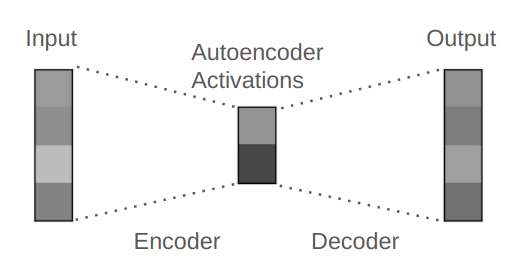
\includegraphics[width=0.5\linewidth]{\toplevelprefix/chapters/chapter5/figs/autoencoder.png}
  \caption{Illustration of a typical autoencoder such as PCA, seeking
  a low-dimensional representation $\bm{z}$ of high-dimensional data $\vx$.}
  \label{fig:AE}
\end{figure}

As we saw in Chapter \ref{ch:classic}, when the distribution of $\vx$ is indeed
supported on a low-dimensional subspace $\vU_o$, the compactness of
the representation
$\vz$ produced by $\cE$ is a direct consequence of correctly
estimating (and enforcing) the dimension of this subspace.  Finally,
recall that gradient descent on the reconstruction criterion exactly
yields these sample-wise consistent mappings: indeed, the optimal
solution to the problem
\begin{equation}\label{eq:pca-reconstruction-ch5}
  \min_{\vU^\top \vU = \vI}\, \bE_{\vx}\left[\norm*{\vx
  - \vU\vU^\top \vx}_2^2\right]
\end{equation}
precisely coincides with $\vU_o$ when the dimension of the representation is
sufficiently large. In this case, we obtain sample-wise consistency
for free, since this guarantees that $\vU_o\vU_o^\top \vx = \vx$.
Notice that in the case of PCA, the rate reduction term in
\eqref{eqn:autoencode-objective-ch5} becomes void as the regularization
on the representation $\Z$ sought is explicit: It spans the entire
subspace of lower dimension\footnote{One may view $\Delta R = 0$ in this case.}.

\paragraph{Online PCA.} Notice that in the above construction, the
linear transform $\vU$
used for the encoding and decoding is computed ``offline'' from all
the input data before hand. One question is whether this transform
can be learned ``online'' as the input data come in order? This
question was answered by the work of Oja in 1982 \cite{Oja1982SimplifiedNM}.
\begin{example}[Normalized Hebbian learning scheme for PCA] Consider a
  sequence of i.i.d. random vectors $\x_1, \ldots, \x_i, \ldots \in
  \mathbb{R}^n$ with covariance $\boldsymbol{\Sigma} \in
  \mathbb{R}^{n\times n}$. Let $\vu_0 \in \mathbb{R}^n$ and define
  the response of an input vector $\x_i$ against a weight vector
  $\vu_i$ to be their inner product:
  \begin{equation}
    \eta_i = \vu_i^T \x_i
  \end{equation}
  and we update the weight vector according to the following scheme:
  \begin{equation}
    \vu_{i+1} = \frac{\vu_i + \gamma \eta_i \x_i}{\|\vu_i + \gamma
    \eta_i \x_i\|}
    \label{eqn:Hebbian}
  \end{equation}
  for some small gain $\gamma >0$. This update scheme can be viewed
  as a normalized Hebbian scheme, in which the weights of connections
  between neurons become stronger if (products of) both the input
  $\x$ and output $\eta$ are strong. One may view the vector of
  weights $\vu$ are ``learned'' based on a form of feedback from the
  output $\eta$.
  Then, under reasonable assumptions, Oja \cite{Oja1982SimplifiedNM} has 
  shown that $\vu_i$ converges to the eigenvector associated with
  the large eigenvalue of $\boldsymbol{\Sigma}$.
\end{example}

The normalized Hebbian scheme \eqref{eqn:Hebbian} can be interpreted as
a first-order approximation to a \textit{stochastic} projected
gradient descent scheme on
the objective of the problem \eqref{eq:pca-reconstruction-ch5} (with batch size
$1$, and with the number of columns of $\vU$ equal to $1$) as long as
$\norm{\vu}_2 = 1$, which is maintained by the projection operation in
\eqref{eqn:Hebbian}.
It is worth keeping its existence in the back of one's mind, both as
a proof of correctness for the use of stochastic gradient methods for
optimizing reconstruction costs such as
\eqref{eq:pca-reconstruction-ch5}, and for its
suggestion that \textit{simpler algorithms than (end-to-end) back
  propagation can
succeed in learning consistent autoencoders}.

\begin{figure}
  \centering
  % \includegraphics[width=12cm]{interpolate.jpg}
  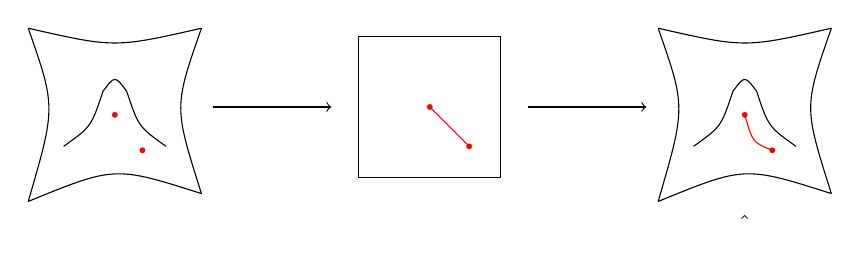
\begin{tikzpicture}
    \draw (-0.1, -0.2) .. controls (1, 0.25) .. (2.1, -0.1);
    \draw (2.1, -0.1) .. controls (1.75, 1) .. (2.1, 2);
    \draw (2.1, 2) .. controls (1, 1.75) .. (-0.1, 2);
    \draw (-0.1, 2) .. controls (0.25, 1) .. (-0.1, -0.2);

    \draw (0.35, 0.5) .. controls (0.7, 0.75) .. (0.85, 1.2);
    \draw (0.85, 1.2) .. controls (1.0, 1.4) .. (1.15, 1.2);
    \draw (1.15, 1.2) .. controls (1.3, 0.75) .. (1.65, 0.5);

    \node[fill, red, circle, inner sep=0.75pt] at (1, 0.9) {};
    \node[fill, red, circle, inner sep=0.75pt] at (1.35, 0.45) {};

    \node at (1, -0.5) {\(\x\)};

    \draw[->] (2.25, 1) -- (3.75, 1);
    \node at (3, 1.25) {\(\fl\)};

    \draw (4.1, 0.1) -- (5.9, 0.1);
    \draw (5.9, 0.1) -- (5.9, 1.9);
    \draw (5.9, 1.9) -- (4.1, 1.9);
    \draw (4.1, 1.9) -- (4.1, 0.1);

    \node[fill, red, circle, inner sep=0.75pt] at (5, 1) {};
    \node[fill, red, circle, inner sep=0.75pt] at (5.5, 0.5) {};

    \draw[red] (5, 1) -- (5.5, 0.5);

    \node at (5, -0.5) {\(\z\)};

    \draw[->] (6.25, 1) -- (7.75, 1);
    \node at (7, 1.25) {\(\re\)};

    \draw (7.9, -0.2) .. controls (9, 0.25) .. (10.1, -0.1);
    \draw (10.1, -0.1) .. controls (9.75, 1) .. (10.1, 2);
    \draw (10.1, 2) .. controls (9, 1.75) .. (7.9, 2);
    \draw (7.9, 2) .. controls (8.25, 1) .. (7.9, -0.2);

    \draw (8.35, 0.5) .. controls (8.7, 0.75) .. (8.85, 1.2);
    \draw (8.85, 1.2) .. controls (9.0, 1.4) .. (9.15, 1.2);
    \draw (9.15, 1.2) .. controls (9.3, 0.75) .. (9.65, 0.5);

    \node[fill, red, circle, inner sep=0.75pt] at (9, 0.9) {};
    \node[fill, red, circle, inner sep=0.75pt] at (9.35, 0.45) {};

    \draw[red] (9, 0.9) .. controls (9.1, 0.55) .. (9.35, 0.45);

    \node at (9, -0.5) {\(\hat{\x}\)};
  \end{tikzpicture}
  \caption{A depiction of interpolation through manifold flattening
    on a manifold in \(\R^{3}\) of dimension \(d = 2\). To interpolate
    two points on the data manifold, map them through the flattening
    map \(\fl\) to the flattened space, take their convex interpolants,
    and then map them back to the data manifold through the
  reconstruction map \(\re\).}
  \label{fig:idealized_interpolation}
\end{figure}

\subsection{Nonlinear PCA and Autoencoding}\label{sub:nonlinear-pca}\label{sec:NLPCA}
Of course, one should expect that things will no longer be so simple
when we deal with more complex distributions whose underlying
low-dimensional structure could be nonlinear.

\paragraph{Data on a Nonlinear Submanifold.} So, to move beyond the
linear structure addressed by PCA, we may assume that the data distribution lies on a (smooth) submanifold $\mathcal{M}$. The intrinsic dimension of the submanifold, say $d$, is typically much lower than the
dimension of the ambient space $\mathbb{R}^D$. From this geometric
perspective, we typically want to find a nonlinear mapping $f$ such that
the resulting manifold
$f(\mathcal{M})$ is flattened, as illustrated by the example shown in Figure
\ref{fig:idealized_interpolation}. The resulting feature $\vz$-space
is typically
more compact (of lower-dimension) than the $\vx$-space, and the
manifold is flat.
From the statistical perspective, which is complementary to the geometric
perspective but distinct in general, we may also want to ensure that the data
distribution on $\cM$ is mapped to a sufficiently regular
distribution, say a Gaussian or a uniform distribution (with a 
very low-dimensional support), in the $\vz$-space. These two properties ensure that sampling and interpolation in the $\vz$-space are as easy as possible, and they are mathematical formalizations of the desirable
notions of compact and structured features in the low-dimensional manifold
model for the data distribution.
In general, the problem of learning such an autoencoding mapping for this class
of data distributions is known as {\em nonlinear principal component analysis}
(NLPCA).

\paragraph{A Classical Attempt via a Two-Layer Network.} As we have
seen above, in the case of PCA, a one-layer linear neural
network is sufficient. That is no longer the case for NLPCA. In 1991, Kramer
\cite{Kramer1991NonlinearPC}  proposed to solve NLPCA by using a two-layer
neural network to represent the encoder mapping $f$ (or its inverse $g$) based
on the universal representation property of two-layer networks with sigmoid
activation:
\begin{equation}
  \z = \vW_2 \sigma(\vW_1\x +\vb),
\end{equation}
where $\sigma(\spcdot)$ is the sigmoid function:
\begin{equation}
  \sigma(x) = \frac{1}{1+ e^{-x}}.
\end{equation}
Cybenko \cite{Cybenko1989ApproximationBS} showed that functions of
the above form (with enough hidden nodes) can approximate any smooth
nonlinear function, say the encoder $f(\spcdot)$, to an arbitrary
precision. In particular, they can represent the flattening and reconstruction
maps for data distributions supported on (unions of) low-dimensional manifolds,
as in \Cref{fig:idealized_interpolation}. The overall architecture of the
original networks proposed by Kramer is illustrated in Figure \ref{fig:NLPCA}.
\begin{figure}[tb]
  \centering
  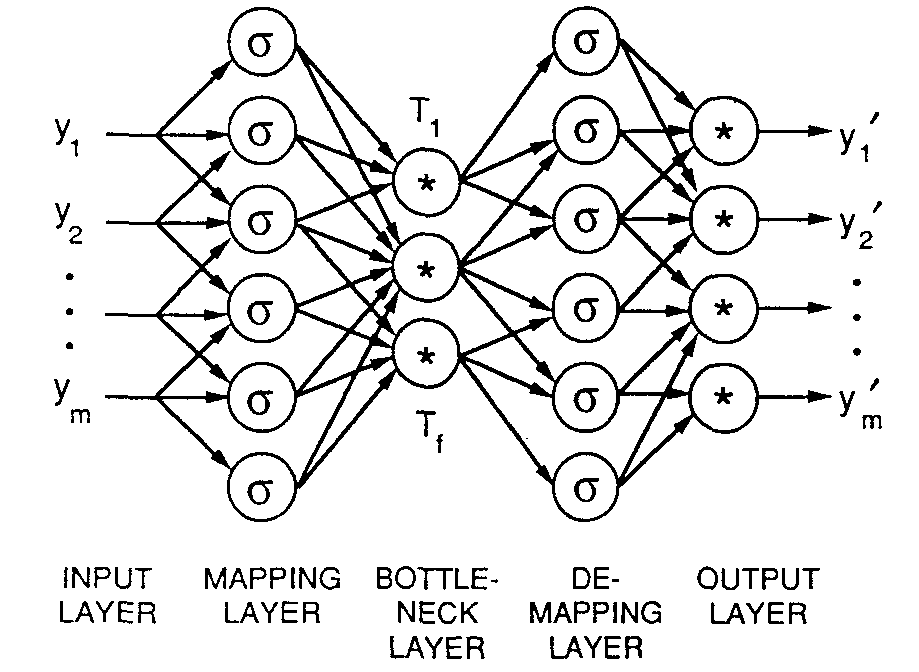
\includegraphics[width=0.6\linewidth]{\toplevelprefix/chapters/chapter5/figs/kramer1991nonlinearPCA.png}
  \caption{Nonlinear PCA by  autoassociative neural networks of depth
    two for both the encoding and decoding mappings, suggested by
  Kramer \cite{Kramer1991NonlinearPC}.}
  \label{fig:NLPCA}
\end{figure}

Unfortunately, unlike the above case of PCA, there is in general no
closed-form learning scheme for the parameters $\boldsymbol{\theta} =
(\vW, \vb)$ of these networks. Hence it was proposed to train the
network via back propagation with the supervision of reconstruction error:
\begin{equation}\label{eq:nonlinear-pca-ch5}
  \min_{\boldsymbol{\theta}} \mathbb{E}[ \|\x - \x'(\boldsymbol{\theta})\|^2].
\end{equation}
Compared to the simple case of PCA, we utilize the same reconstruction objective
for learning, but a far more complex nonlinear class of models for
parameterizing and learning the encoder and decoder. Although universal
approximation properties such as Cybenko's suggest that \textit{in principle}
learning consistent autoencoders via this framework is possible---because for
any random sample of data, given enough parameters, such autoencoding pairs
exist---one often finds it highly nontrivial to find them with gradient descent.
Moreover, to obtain an informative enough reconstruction objective
and model for the
distribution of high-dimensional real-world data such as images, the required
number of samples and hidden nodes can be huge.
In addition, as a measure of the compactness of the learned representation, the
(lower) dimension of $\z$ for the bottleneck layer is often chosen
heuristically.\footnote{In the later work \cite{Hinton-1993}, Hinton et.
  al. suggested to use the minimum description length (MDL) principle to promote
  the compactness of the learned coding scheme, in a spirit very similar to the
rate distortion measure introduced in this book.}
% \sdb{We can connect to Oja's here too: we learn with BP (don't just call GD)
% + it becomes nonlocal...}

\paragraph{Manifold Flattening via a Deeper Network.}
Based on the modern practice of deep networks, such classical shallow
and wide network architectures are known to be rather difficult to
train effectively and efficiently via back propagation (BP), partly
due to the diminishing gradient of the sigmoid function. Hence, the
modern practice normally suggests to further
decompose the nonlinear transform $f$ (or $g$) into a composition of
many more layers of simpler transforms, resulting a deeper network architecture
\cite{Hinton504}, as illustrated in Figure \ref{fig:ccnet_layers}.
In the modern context, further elaborations over the basic reconstruction cost
\eqref{eq:nonlinear-pca-ch5} also prove necessary to achieve good performance on
complex real-world data distributions such as images.

\begin{figure}[htb]
  \centering
  \begin{tikzpicture}
    \draw (-0.1, -0.2) .. controls (1, 0.25) .. (2.1, -0.1);
    \draw (2.1, -0.1) .. controls (1.75, 1) .. (2.1, 2);
    \draw (2.1, 2) .. controls (1, 1.75) .. (-0.1, 2);
    \draw (-0.1, 2) .. controls (0.25, 1) .. (-0.1, -0.2);

    \draw (0.35, 0.5) .. controls (0.7, 0.75) .. (0.85, 1.2);
    \draw (0.85, 1.2) .. controls (1.0, 1.4) .. (1.15, 1.2);
    \draw (1.15, 1.2) .. controls (1.3, 0.75) .. (1.65, 0.5);

    \node at (1, -0.5) {\(\x\)};

    \draw[->] (2.25, 1.25) -- (3.25, 1.25);
    \node at (2.75, 1.5) {\(\fl_{1}\)};

    \draw[->] (3.5, 1.25) -- (4.5, 1.25);
    \node at (4, 1.5) {\(\fl_{2}\)};

    \draw[->] (4.75, 1.25) -- (5.75, 1.25);
    \node at (5.25, 1.5) {\(\cdots\)};

    \draw[->] (6, 1.25) -- (7, 1.25);
    \node at (6.5, 1.5) {\(\fl_{L}\)};

    \draw[->] (7, 0.75) -- (6, 0.75);
    \node at (6.5, 0.5) {\(\re_{L}\)};

    \draw[->] (5.75, 0.75) -- (4.75, 0.75);
    \node at (5.25, 0.5) {\(\cdots\)};

    \draw[->] (4.5, 0.75) -- (3.5, 0.75);
    \node at (4, 0.5) {\(\re_{2}\)};

    \draw[->] (3.25, 0.75) -- (2.25, 0.75);
    \node at (2.75, 0.5) {\(\re_{1}\)};

    \draw (7.3, 0.1) -- (9.1, 0.1);
    \draw (9.1, 0.1) -- (9.1, 1.9);
    \draw (9.1, 1.9) -- (7.3, 1.9);
    \draw (7.3, 1.9) -- (7.3, 0.1);

    \node at (8.2, -0.5) {\(\z\)};

  \end{tikzpicture}
  \caption{A depiction of the construction process of the flattening
    and reconstruction pair \((\fl, \re)\), where the encoder \(\fl =
    \fl_{L} \circ \fl_{L - 1} \circ \cdots \circ \fl_{1}\) is
    constructed from composing flattening layers, and the decoder \(\re
    = \re_{1} \circ \re_{2} \circ \cdots \circ \re_{L}\) is composed of
  inversions of each \(\fl_{\ell}\).}
  \label{fig:ccnet_layers}
\end{figure}

In light of universal approximation theorems such as Cybenko's, one
may initially wonder why, conceptually, deeper autoencoders should be preferred
to shallow ones.
From purely an expressivity perspective, we can understand this phenomenon
through a geometric angle related to the task of flattening the nonlinear
manifold on which our hypothesized data distribution is supported. A purely
constructive approach to flattening the manifold proceeds incrementally, in
parallel to what we have seen in \Cref{ch:compression,ch:representation} with
the interaction between diffusion, denoising, and compression. In the geometric
setting, the incremental \textit{flattening process} corresponding to $f_{\ell}$
takes the form of transforming a neighborhood of one point of the manifold to be
closer to a flat manifold (i.e., a subspace), and enforcing local consistency
with the rest of the data samples; the corresponding incremental operation in
the decoder, $g_{\ell}$, undoes this transformation. This procedure precisely
incorporates curvature information about the underlying manifold, which is
estimated from data samples. Given enough samples from the manifold and
a careful instantiation of this conceptual process, it is possible to implement
this procedure as a computational procedure that verifiably flattens nonlinear
manifolds in a white-box fashion \cite{Psenka-JMLR24}. However, the approach is
limited in its applicability to high-dimensional data distributions such as
images due to unfavorable scalability, motivating the development of more
flexible methods to incremental autoencoding.

\subsection{Sparse Autoencoding}
In the above autoencoding schemes, the dimension of the feature space
$d$ is typically chosen to be much lower than that the original data
space $D$ so as to explicitly enforce or promote the learned
representation to be low-dimensional. However, in practice, we
normally do not know the intrinsic dimension of the data
distribution. Hence, the choice of the feature space dimension for
autoencoding is often done empirically. In more general situations,
the data distribution can be a mixture of a few low-dimensional
subspaces or submanifolds. In these cases, it is no longer feasible
to enforce a single low-dimensional space for all the features together.

The sparse autoencoder is meant to resolve some of these limitations. In
particular, the dimension of the feature space can be equal to or
even higher than that of the data space, as illustrated in Figure
\ref{fig:SAE}. However, the features are required to be highly
sparse in the feature space. So if we impose sparsity as the measure
of parsimony in addition to the rate reduction in the objective
\eqref{eqn:autoencode-objective-ch5}, we obtain a new objective for
the sparse autoencoding:
\begin{equation}
  \min_{f, g}
  %\lambda
  \|\Z\|_0 - \Delta R_{\epsilon}(\Z) + d(\X, \hat \X),
  \label{eqn:autoencode-sparse}
\end{equation}
where the $\ell^0$-``norm'' $\|\spcdot\|_0$ is known to promote sparsity.
This is very similar to the sparse rate reduction objective
\eqref{eq:sparse-rr} which we used in the previous Chapter \ref{ch:representation} to derive the white-box CRATE architecture.

\begin{figure}
  \centering
  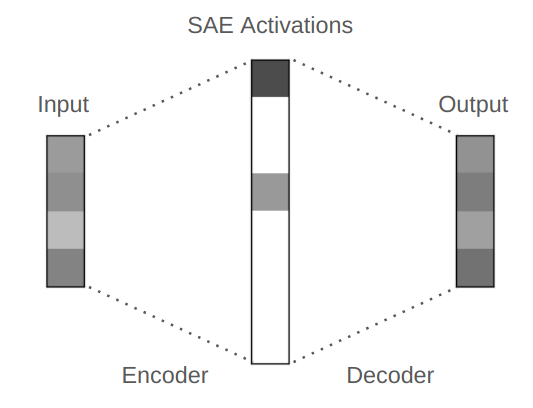
\includegraphics[width=0.5\linewidth]{\toplevelprefix/chapters/chapter5/figs/SAE_diagram.png}
  \caption{Illustration of a sparse autoencoder (SAE), compared to
  that of a typical autoencoder (AE) in Figure \ref{fig:AE}. }
  \label{fig:SAE}
\end{figure}

%\yima{There are other ways to promote the sparsity of the learned
% features $\Z$, including enforcing the frequency of activations for
%  each coordinate of $\z$ to be small... But here we can justify SAE
%  through its natural connection to sparse rate reduction. Anthropic
% AIseems to advocate that sparse autoencoding learns more
% interpretable features... }

As a method for learning autoencoding pairs in an end-to-end fashion, sparse
autoencoding has been practiced in the past \cite{Ranzato2006-oq}, but nearly
all modern autoencoding frameworks instead use a different, probabilistic
autoencoding framework, which we will study shortly.
However, it is worth noting that a significant amount of attention has been
devoted in recent years to training sparse autoencoders for the purpose of
\textit{interpreting features in pretrained large-scale deep networks}, such as
transformers, following the hypothesis that the (non-interpretable, \textit{a
priori}) features in these networks consist of sparse ``superpositions'' of
underlying features, which are themselves interpretable
\cite{elhage2022superposition}.
It is illuminating to contrast this methodology with the classical sparse
autoencoding framework, and with the general autoencoding methodology we have
laid out in this Chapter.
In the most straightforward instantiation of sparse autoencoder training and
evaluation (see \citep{huben2024sparse, gao2025scaling}),
a large number of features from a pretrained deep network $h$ are collected from
different inputs $\vx_i$, which themselves are chosen based on a desired
interpretation task.\footnote{For example, the inputs $\vx_i$ could correspond
  to texts containing samples of computer code in different
  programming languages,
  with our task being to try to identify interpretable features in a transformer
  feature map $h$ corresponding to different salient aspects of the
  input, such as
  the
  specific programming language (distinct across input ``classes'')
  or the need to
  insert a matching parenthesis at the current position (common
  across input ``classes''). We
  discuss the
  use of deep networks, and in particular transformers, for text representation
learning in greater detail in \Cref{ch:applications}.} For
simplicity, we will use $h$ to denote the pre-selected feature map in question,
with $D$-dimensional features; given $N$ sample inputs, let $\vH \in \bR^{D
\times N}$ denote the full matrix of features of $h$.
Then a sparse autoencoder $f : \bR^D \to \bR^d$, with decoder $g : \bR^d \to
\bR^D$, is trained via the relaxed version of the objective in
\Cref{eqn:autoencode-sparse}:
\begin{equation}\label{eq:sae-loss}
  \min_{f, g}
\lambda \|f(\vH)\|_1 + \frac{1}{2} \| \vH - g(f(\vH))) \|_2^2,
\end{equation}
where the sparse autoencoder $f$ commonly takes the form of a one-layer neural
network, i.e.\ $f(\vh_i) = \sigma(\vW_{\mathrm{enc}}(\vh_i - \vb)
+ \vb_{\mathrm{enc}})$, where $\sigma(x) = \max \{x, 0\}$ is the ReLU activation
function, and the decoder $g$ is linear, so that $g(\vz_i)
= \vW_{\mathrm{dec}}\vz + \vb$.
Interestingly, these simple architectures for the sparse autoencoder and decoder
can be seen as exactly analogous to those that would be obtained from the
unrolled optimization approach we have expounded in \Cref{ch:representation},
and in particular to the CRATE architecture's ISTA block
(see \eqref{eq:ista-block}).
More precisely, the sparse autoencoder's encoder can be seen as one step of
proximal gradient descent on the nonnegative LASSO objective, which, as we have
seen, leads to the CRATE ISTA block; the asymmetric structure of the encoder and
decoder can be similarly understood as the difference between the forward
mapping in the ISTA block (see \eqref{eq:ista-block}) and the sparsifying
dictionary $\vD$ itself, which becomes the decoder.
This connection suggests a host of new design strategies for improving the
representation ability of sparse autoencoders, few of which seem to have been
thoroughly explored thus far.

\subsection{Variational Autoencoding}\label{sec:vae}

In the classical conception of autoencoding, following Hinton and Rumelhart
\cite{Rumelhart1986}, the data distribution plays a very minor role in the
formulation, in spite of its centrality to the representation we ultimately
learn. Indeed, in the naive framework, one hopes that by training a deep network
to reconstruct samples from the data distribution with a suitably-configured
bottleneck for the representation $\vz$, the learned encoders $f$ and $g$ will
naturally end up corresponding to a compact and structured feature
representation for the data. This is rarely the case in practice.
An improved, more modern methodology for autoencoding that still finds
significant application to this day is \textit{variational autoencoding}
\cite{Kingma2013-sb,Kingma2019-zh}.
We will see how this framework, which trains a variational autoencoder (VAE)
derived through probabilistic modeling considerations, both generalizes the
classical autoencoder training (via minimization of the reconstruction loss),
and stabilizes it with appropriate regularization. Later, we will see how to
begin to go further and go beyond the black-box nature of the deep networks used
to represent the encoding and decoding mappings $f$ and $g$.

\subsubsection{Probabilistic Perspective on Autoencoding}
In the manifold model for the data distribution, the key mathematical objects
are the \textit{support} of the data distribution, namely the manifold $\cM$,
and the density of the data on the support, say $p$. When we formulate
autoencoding from the probabilistic perspective, we often think of the
high-dimensional input $\vx$ as having a density $p$ with support on $\R^D$; one
can think of adding a very small amount of noise to the (degenerate)
distribution supported on the manifold $\cM$ to obtain this density $p$, in line
with our denoising-diffusion constructions in Chapter \ref{ch:compression}.
Then the goal of generative probabilistic modeling is to learn the density $p$
from samples $\vx$, say from a class of models $p(\vx;\, \vtheta)$ parameterized
by $\vtheta$. As we have recalled in Chapter \ref{ch:compression}, a classical
approach to achieving this is via maximum likelihood estimation:
\begin{equation*}\label{eq:VAE-MLE}
\max_{\vtheta}\, \bE_{\vx}[ \log p(\vx;\, \vtheta) ].
\end{equation*}
For certain representative classes of data distributions $p$ %
% , including the
% manifold model without any further geometric constraints
% \cite{kiani2024hardness},
and sufficiently-expressive classes of models $p(\vx;\, \vtheta)$, even simpler
learning problems than the maximum likelihood estimation problem are known to be
statistically hard \cite{Yang1999-wb}. Hence it is desirable to exploit the
knowledge that $\vx$ has low-dimensional structure by seeking to factor the
distribution $p(\vx ;\, \vtheta)$ according to a low-dimensional ``latent''
variable model $\vz$. Indeed, we may write by conditioning $p(\vx,
\vz ;\, \vtheta)
= p(\vz;\, \vtheta) p(\vx \mid \vz;\, \vtheta)$, and
\begin{align*}
p(\vx; \vtheta) &= \int p(\vz;\, \vtheta) p(\vx \mid \vz;\, \vtheta) \odif \vz
\\
&=
\bE_{\vz \sim p(\,\cdot\,;\, \vtheta)}[ p(\vx \mid \vz;\, \vtheta) ].
\end{align*}
Classically, our model for the data distribution $p(\vx;\, \vtheta)$ corresponds
to a choice of the latent distribution $p(\vz;\, \vtheta)$ and the conditional
distribution $p(\vx \mid \vz;\, \vtheta)$.
Even so, computing the model for the data distribution from these latent
distributions is intractable except for in special cases, analogous to those we
have studied in Chapter \ref{ch:classic}.
By the same token, computing the posterior $p(\vz \mid \vx;\, \vtheta)$ from
data, allowing us to \textit{encode} samples to their corresponding latents, is
generally intractable.
There is hence a tradeoff between the expressivity of our generative model,
its computational tractability, and the accuracy of any approximations we make
to the underlying probabilistic framework for the sake of
computational tractability.
In navigating this tradeoff, one also needs a flexible computational approach
for learning the model parameters $\vtheta$ from data, analogous to the maximum
likelihood objective.

In the variational autoencoding framework, we navigate this tradeoff through
three key insights:
\begin{enumerate}
\item We posit \textit{simple} distributions for $\vz$ and $\vx$ conditional
  on $\vz$, but make their parameters depend in a highly flexible way on the
  input data $\vx$ (where relevant) using deep networks.
\item We replace the posterior $p(\vz \mid \vx;\, \vtheta)$, used for encoding
  and whose form is implied (by Bayes rule) by our modeling choices for $\vz$,
  with a tractable approximation $q(\vz \mid \vx;\, \veta)$, which has its own
  parameters $\veta$.
\item We jointly learn $\vtheta$ and $\veta$ via maximizing a tractable lower
  bound for the likelihood $p(\vx ;\, \vtheta)$, known as the evidence lower
  bound (ELBO).
\end{enumerate}
We will focus on the most useful instantation of the VAE framework
for practice, namely
where the prior $p(\vz ;\, \vtheta)$ and the conditional $p(\vx \mid \vz;\,
\vtheta)$ are both Gaussian. Namely, we use the following Gaussian
distributions:
\begin{align*}
\vz &\sim \cN(\Zero, \vI), \\
\vx \mid \vz &\sim \cN(g_1(\vz), \diag(e^{g_2(\vz)}) \vI),
\end{align*}
where $g = (g_1, g_2)$ are deep networks with parameters $\vtheta$, which
correspond to the \textit{decoder} in the autoencoder.
Similarly, for the approximate posterior $q(\vz \mid \vx;\, \veta)$, we use
a special Gaussian distribution with parameters given by an encoder
MLP $f = (f_1, f_2)$ with parameters $\veta$:
\begin{equation*}
\vz \mid \vx \sim \cN(f_1(\vx), \diag(e^{f_2(\vx)}) \vI).
\end{equation*}
%\yima{We might need to elucidate what are the true implications of
% the above two assumptions on the forms of the two conditional
% distributions. How do these assumptions enforce certain desired
% structures of the representation and how are the structures related
% to what rate reduction and sparsity are promoting? }
This makes probabilistic encoding and decoding simple: we simply map our data
$\vx$ to mean and variance parameters of a Gaussian distribution for
encoding, or vice versa.
For learning the encoder and decoder, we start from the maximum likelihood
objective \Cref{eq:VAE-MLE}, and derive a convenient lower bound known as the
evidence lower bound, or ELBO. Starting from simple algebraic manipulations
\begin{align*}
\log p(\vx;\, \vtheta) &=
\log \frac{p(\vx, \vz;\, \vtheta)}{p(\vz \mid \vx;\, \vtheta)}
\\
&=
\log \frac{p(\vx, \vz;\, \vtheta)}{q(\vz \mid \vx;\, \veta)}
+
\log \frac{q(\vz \mid \vx;\, \veta)}{p(\vz \mid \vx;\, \vtheta)},
\end{align*}
we take expectations with respect to $\vz \sim q(\,\cdot\, \mid
\vx;\, \veta)$ and
use the Gibbs inequality (\Cref{thm:information-inequality}) to get
\begin{equation*}
\log p(\vx;\, \vtheta)
\geq
\bE_{\vz \sim q(\,\cdot\, \mid \vx ;\, \veta)} \left[
  \log \frac{p(\vx, \vz;\, \vtheta)}{q(\vz \mid \vx;\, \veta)}
\right].
\end{equation*}
The righthand side of this bound is the ELBO; as a lower bound for the pointwise
log-likelihood of $p(\vx;\, \vtheta)$, its maximization offers a
principled compromise
between the maximum likelihood objective and computational tractability.
Interestingly, the derivation above shows that its tightness depends on the KL
divergence between the approximate posterior $q(\vz \mid \vx;\, \veta)$ and the
true posterior $p(\vz \mid \vx;\, \vtheta)$, implying that the more accurate our
approximate posterior is, the more maximization of the ELBO leads to
maximization of the underlying objective of interest, the likelihood of the
data. Thus, the VAE objective is:
\begin{equation}\label{eq:elbo-objective}
\max_{\vtheta, \veta}\,
\bE_{\vx}
\bE_{\vz \sim q(\,\cdot\, \mid \vx ;\, \veta)} \left[
  \log \frac{p(\vx, \vz;\, \vtheta)}{q(\vz \mid \vx;\, \veta)}
\right].
\end{equation}
By our derivation, maximization of this objective corresponds to a tradeoff
between maximizing the likelihood function of the data and minimizing the KL
divergence between the approximate and true posterior, which is a highly
sensible objective given the VAE modeling assumptions.

\subsubsection{VAE Training as Probabilistic Autoencoding}

There is a general methodology for maximizing the ELBO objective in
\Cref{eq:elbo-objective} using stochastic gradient descent and various tractable
Monte Carlo estimators for the associated gradients. However, the task is
simpler under the Gaussian assumptions we have made above. In this case, the
ELBO reads
\begin{align*}
&\max_{\vtheta, \veta}\,
\bE_{\vx}
\bE_{\vz \sim q(\,\cdot\, \mid \vx ;\, \veta)} \left[
  \log \frac{p(\vx, \vz;\, \vtheta)}{q(\vz \mid \vx;\, \veta)}
\right]\\
=&
\max_{\vtheta, \veta}\,
\left\{
  \bE_{\vx}
  \bE_{\vz \sim q(\,\cdot\, \mid \vx ;\, \veta)} \left[
    \log p(\vx, \vz;\, \vtheta)
  \right]
  + \frac{d \log(2\pi e)}{2}
  % + \frac{1}{2}\sum_{i=1}^d f_{2, i}(\vx)
  + \frac{1}{2} \ip{ \bE_{\vx}[f_2(\vx)]}{\mathbf{1}}
\right\}
\\
\equiv &
\max_{\vtheta, \veta}\,
\left\{
  \bE_{\vx}
  \bE_{\vz \sim q(\,\cdot\, \mid \vx ;\, \veta)} \left[
    \log p(\vx \mid \vz;\, \vtheta)
    + \log p(\vz)
  \right]
  % +
  % \bE_{\vz \sim q(\,\cdot\, \mid \vx ; \veta)} \left[
  %   \log p(\vz)
  % \right]
  % + \frac{1}{2}\sum_{i=1}^d f_{2, i}(\vx)
  + \frac{1}{2} \ip{ \bE_{\vx}[f_2(\vx)]}{\mathbf{1}}
\right\}
\\
\equiv &
\max_{\vtheta, \veta}\,
\left\{
  2\bE_{\vx}\left[
    \bE_{\vz \sim q(\,\cdot\, \mid \vx ;\, \veta)} \left[
      \log p(\vx \mid \vz;\, \vtheta)
    \right]
    + \ip{ f_2(\vx) - e^{f_2(\vx)}}{\mathbf{1}}
    - \norm{f_1(\vx)}_2^2
    % + \frac{1}{2}\sum_{i=1}^d \left(
    %   f_{2, i}(\vx) - f_{1, i}^2(\vx) - e^{f_{2, i}(\vx)}
    % \right)
  \right]
\right\}, \labelthis \label{eq:elbo-for-gaussians}
\end{align*}
following \Cref{thmx:max_entropy} and the Gaussian entropy calculation done in \Cref{app:diffusion-denoising}, where $\equiv$
denotes equivalence of optimization objectives (in each case, we remove some
additive constants that do not change the optimization problem's solutions).
The remaining term corresponds to the ``autoencoding'' part of the ELBO
objective: intuitively, it seeks to maximize the likelihood of data generated by
the decoder when the latents $\vz$ are distribited according to the approximate
posterior (generated by the encoder applied to a data sample $\vx$), which is
a probabilistic form of autoencoding.
To see this more directly, consider the special case where the approximate
posterior concentrates on its mean $f_1(\vx)$, for every $\vx$: this
is the limit
where its log-variance $f_{2,i}(\vx) \to -\infty$ for each coordinate
$i = 1, \dots, d$.
For simplicity, assume moreover that $g_2(\vx) = \mathbf{1}$, giving the decoder
constant unit variance on each coordinate.
Then the loss term in question converges to
\begin{align*}
\bE_{\vx}
\bE_{\vz \sim q(\,\cdot\, \mid \vx ;\, \veta)} \left[
  \log p(\vx \mid \vz;\, \vtheta)
\right]
&\to
\bE_{\vx} \left[
  \log p(\vx \mid f_1(\vx);\, \vtheta)
\right]
\\
% &=
% -\frac{1}{2} \bE_{\vx} \left[
%   (\vx - g_1\circ f_1(\vx))^\top \diag(e^{g_2\circ
% f_1(\vx)})^{-1} (\vx - g_1
%   \circ f_1(\vx))
%   % + \logdet\left( 2\pi \diag(e^{g_2 \circ f_1(\vx)}) \right)
%   + \sum_{i=1}^D (g_2 \circ f_1)_i(\vx)
% \right].
&\equiv
-\frac{1}{2} \bE_{\vx} \left[
  \|\vx - g_1\circ f_1(\vx)\|_2^2
\right].
\end{align*}
So with a highly confident encoder, which deterministically maps each sample
$\vx$ to a single point $f_1(\vx)$ in $\vz$-space, and an isotropic decoder,
the ``autoencoding'' part of the ELBO maximization problem indeed becomes
a classical autoencoding objective!\footnote{In the general case where $g_2$ is
not fixed as $\mathbf{1}$, the reader can verify that the autoencoding term in
the ELBO objective converges to a \textit{regularized} classical autoencoding
objective.}
At the same time, note that this special case is actually excluded by the
extra terms in \Cref{eq:elbo-for-gaussians}---these effectively correspond to
regularization terms that discourage the encoder from collapsing.
The general ELBO loss (\Cref{eq:elbo-objective,eq:elbo-for-gaussians}) is
therefore a strict generalization of the classical autoencoding reconstruction
objective (\Cref{eq:nonlinear-pca-ch5}), both in terms of its data fidelity term
and in terms of the inclusion of regularization terms.

\subsubsection{Training a VAE}
VAEs are typically trained by alternating stochastic gradient ascent on the ELBO
objective (\Cref{eq:elbo-for-gaussians}), given individual samples
$\vx$ from the
true data distribution and from $\vz \sim q(\,\cdot\,\mid \vx;\, \veta)$. In
particular, it is standard to collect and train on many independently-generated
samples $\vz^{i}$ for each sample $\vx$. To take gradients of
\Cref{eq:elbo-for-gaussians} with respect to the encoder parameters $\veta$,
one makes use of the so-called reparameterization trick by writing $\vz \sim
q(\,\cdot\,\mid \vx;\, \veta)$ as
\begin{equation*}
\vz =_{\mathrm{d}} f_1(\vx) + \diag(e^{\tfrac{1}{2}f_2(\vx)}) \vg,
\quad \vg \sim
\cN(0, \vI),
\end{equation*}
where $=_{\mathrm{d}}$ denotes equality in distribution. Then one can simply
take many independent standard Gaussian samples $\vg^{i}$ for each data sample
$\vx$, generate the corresponding samples from the approximate posterior
$\vz^i$, and compute gradients with respect to $\veta$ using automatic
differentiation without any issues.


%The previous Chapter 6:

\section{Learning Self-Consistent Representations}
\label{sec:self-consistency}

In earlier chapters, we have studied methods that would allow us to learn a low-dimensional distribution via (lossy) compression. As we have mentioned in Chapter \ref{ch:intro} and demonstrated in the previous chapters, the progresses made in machine intelligence largely rely on finding computationally feasible and efficient solutions to realize the desired compression, not only computable or tractable in theory, but also scalable in practice:
\begin{equation}
\mbox{\textbf{computable}} \;
   \Longrightarrow \; \mbox{\textbf{tractable}} \; \Longrightarrow \; 
   \mbox{\textbf{scalable}}.
\end{equation}
It is even fair to say that the tremendous advancement in machine intelligence made in the past decade or so is largely attributed to the development of scalable models and methods, say by training deep networks via back propagation. Large models with billions of parameters trained with trillions of data points on tens of thousands of powerful GPUs have demonstrated super-human capabilities in memorizing existing knowledge. This has led many to believe that the ``intelligence'' of such models will continue to improve as their scale continues to go up. 

While we celebrate the engineering marvels of such large man-made machine learning  systems, we also must admit that, compared to intelligence in nature, this approach to improve machine intelligence is unnecessarily resource demanding. Natural intelligent beings, including animals and humans, simply cannot afford such a brute force solution to learn because they must operate with a very limited budget in energy, space and time, subject to many strict physical constraints. 

Firstly, there is strong scientific evidence that our brain does not conduct global end-to-end back propagation to improve or correct its predictions. Instead, it was long known in neuroscience that our brain corrects errors with local closed-loop feedback, such as predictive coding. This was the scientific basis that had inspired Norbert Wiener to develop the theory of feedback control and the Cybernetics program back in the 1940s. 

Secondly, we saw in the previous sections that in order to learn a consistent representation, one needs to learn a bi-directional autoencoding:
\begin{equation}
 \X
\xrightarrow{\hspace{1mm} \mathcal{E} = f \hspace{1mm}} \Z  \xrightarrow{\hspace{1mm} \mathcal{D} = g \hspace{1mm}} \hat{\X}.
\end{equation}
It requires to enforce the observed input data $\X$ and the decoded $\hat \X$ to be close by some measure of similarity $d(\X, \hat \X)$. In nature, animals or humans rarely have direct assess to the ground truth $\X$. For example, we never have direct access to true 3D shape, distance, or dynamics of objects in a scene. Yet, we have all learned to estimate and predict them very accurately and efficiently. Hence, an outstanding question is how we can learn the true distribution of the $\X$, even though we cannot directly compare our estimate $\hat \x$ with the ground truth $\x$. As we will see in this chapter, the answer also  lies in the closed-loop feedback, as well as the low-dimensionality of the data distribution. 



%This section introduces the concept of self-consistent for a system that learns autonomously.

% \begin{itemize}
%     \item Contrast: supervised representation learning needs human signal (class), self-supervised representation learning needs human signal (masking, augmentation), how to remove human signal from the mixture and get a autonomous system?
%     \item For full autonomy, need to work in both \(x\) space (actions, perceptions) and \(z\) space (representations, compression, planning?)
%     \item Measure distance in \(x\) space? Deficiencies in \(\ell^{2}\) loss, Wasserstein loss, etc 
%     \item Measure distance in \(z\) space? Only possible with compact and structured \(z\) space (say piecewise linear structure, i.e., mixture of subspaces)
%     \item Propose self-consistency: representation is consistent wrt itself --- features are consistent wrt their autoencoding 
% \end{itemize}


As we know from the previous chapter, in order to ensure a representation is consistent, we need to compare the generated $\hat \X \sim p(\hat\x)$ and the original $\X \sim p(\x)$, at least in distribution. Even when we do have access to $\X$ and $\hat \X$, technically, computing and minimizing distance of two distributions can be problematic, especially when the support of the distributions is low-dimensional. The KL-divergence introduced \ref{ch:compression} is not even well-defined between two distributions that do not have overlap supports. 

As an early attempt to alleviate the above difficulty in computing and minimizing the distance between two (low-dimensional)  distributions, people had suggested to learn the generator/decoder $g$ via discriminative approaches \cite{Tu-2007}. This line of thought has led to  the idea of {\em Generative Adversarial Nets (GAN)} \cite{goodfellow2014generative}. It introduces a discriminator $d$, usually modeled by a deep network, to discern differences between the generated samples $\hat \X$ and the real ones $\X$:
\begin{equation}
 \Z \xrightarrow{\hspace{2mm} g(\z,\eta) \hspace{2mm}} \hat \X, \, \X \xrightarrow{\hspace{2mm} d(\x, \theta)\hspace{2mm}} \{\mathbf 0, \mathbf 1\}.
 \label{eqn:GAN}
\end{equation}
It is suggested that we may attempt to align the distributions between $\hat \x$ and $\x$ via a {\em Stackelberg game} between the generator $g$ and the discriminator $d$:
\begin{equation}
\max_{\theta}\min_{\eta} \mathbb{E}_{p({\x})}\big[\log d(\x,\theta)\big] + \mathbb{E}_{p({\z})}\big[1 - \log d(\underbrace{g(\z,\eta)}_{\hat \x \,\sim\, p_g},\theta)\big].
\end{equation}
That is, the discriminator $d$ is trying to minimize the cross entropy between the true samples $\X$ and the generated ones $\hat \X$ while the generator $g$ is trying to do  the opposite. 

One may show that finding an equilibrium for the above Stackelberg game is equivalent to minimizing the {\em Jensen-Shannon divergence}:
\begin{equation}
    \mathcal{D}_{JS}(p(\x), p_g(\hat \x)) = \mathcal{D}_{KL}\big(p \| (p + p_g)/{2}\big) + \mathcal{D}_{KL}\big(p_g \| (p + p_g)/{2}\big).
\end{equation}
Note that, compared to the KL-divergence, the~JS-divergence is well-defined even if the supports of the two distributions are non-overlapping. However, JS-divergence does not have a closed-form expression even between two Gaussians, whereas KL-divergence does. In addition, since the data distributions are low-dimensional, the~JS-divergence can be highly ill-conditioned to optimize.\footnote{as shown in \cite{arjovsky2017wasserstein}.} This may explain why many additional heuristics are typically used in many subsequent variants of GAN. 

So, instead, it has also been suggested to replace JS-divergence with the earth mover (EM) distance or the Wasserstein distance.\footnote{Roughly speaking, for distributions with potentially non-overlapping low-dimensional supports, the JS-divergence behaves like the $\ell^0$-norm, and the EM-distance behaves like the $\ell^1$-norm.} However both JS-divergence and W-distance can only be approximately computed between two general distributions.\footnote{For instance, the W-distance requires one to compute the maximal difference between expectations of the two distributions over all 1-Lipschitz functions.} Furthermore, neither the JS-divergence nor the W-distance have closed-form formulae, even for the Gaussian distributions.\footnote{The ($\ell^1$-norm) W-distance can be bounded by the ($\ell^2$-norm) W2-distance which has a closed-form \cite{salmona2021gromovwasserstein}. However, as is well-known in high-dimensional geometry, $\ell^1$-norm and $\ell^2$ norm deviate significantly in terms of their geometric and statistical properties as the dimension becomes high \cite{Wright-Ma-2021}. The~bound can become very loose.} 

If it is difficult to compare distributions of the data $\X$ and $\hat \X$, would it possible to compare in the learned feature $\Z$ with its image $\hat \Z$ under the encoder $f$: 
\begin{equation}
 \X
\xrightarrow{\hspace{1mm} \mathcal{E} = f \hspace{1mm}} \Z  \xrightarrow{\hspace{1mm} \mathcal{D} = g \hspace{1mm}} \hat{\X} \xrightarrow{\hspace{1mm} \mathcal{E} = f \hspace{1mm}} \hat \Z?
\label{eqn:closed-autoencoding}
\end{equation}
This leads to the notion of {\em self-consistent representation}.
\begin{definition}[Self-Consistent Representation]\label{def:closed_loop}
    Given data \(\vX\), we call an \textit{self-consistent representation} to be a pair of functions \((f \colon \cX \to \cZ, g \colon \cZ \to \cX)\), such that the \textit{features} \(\vZ = f(\vX)\) are compact and structured, and the \textit{autoencoding features} \(\hat{\vZ} \doteq f \circ g(\vZ)\) is \textit{close} to \(\vZ\). 
    \begin{enumerate}
        \item We say that it is \textit{sample-wise} self-consistent if \(\vZ \approx \hat{\vZ}\) in a certain norm  with high probability.
        \item We say that the representation is \textit{distributionally self-consistent} if \(\Law(\vZ) \approx \Law(\hat{\vZ})\).
    \end{enumerate}
\end{definition}


%\section{Closed-Loop Transcription}

\subsection{Closed-Loop Transcription via Stackelberg Games}\label{sec:closed-loop-transcription}
%This subsection introduces the closed-loop transcription framework and the game-theoretic formulation from \href{https://www.mdpi.com/1099-4300/24/4/456/htm}{the CTRL work}.

% \begin{itemize}
%     \item Closed loop transcription framework: feature quality for \(z\) and \(\hat{z}\) plus distance measure for \(z\) and \(\hat{z}\)
%     \item \(f\) plays role as encoder, discriminator, sensor; \(g\) plays role as decoder, generator, controller 
%     \item \(f\) maximizes above objective, \(g\) minimizes 
%     \item optimization strategy: gradient descent-ascent, or two-timescale GDA, or something else?
% \end{itemize}

% \begin{itemize}
%     \item also need to give an intro to game theory somewhere here...
% \end{itemize}

How do we try to ensure a learned representation is self-consistent? As usual, let us assume $\X = \cup_{k=1}^K \X_k$ with each subset of samples $\X_k$ belonging to a low-dimensional submanifold: $\X_k \subset \mathcal{M}_k, k = 1,\ldots, K$. Following the notation in Chapter \ref{ch:general-distribution}, we use a matrix $\bm \Pi_k(i,i) = 1$ to denote the membership of sample $i$ belonging to class $k$ and $\bm \Pi_k(i,j) = 0$ otherwise. One seeks a continuous mapping $f(\cdot,\bm \theta): \x \mapsto \z$ from $\X$ to an optimal representation $\Z = [\z_1, \ldots, \z_N] \subset \Re^{d \times N}$:
\begin{equation}
\bm X  \xrightarrow{\hspace{2mm} f(\x, \bm \theta) \hspace{2mm}} \bm Z, 
\label{eqn:LDR}
\end{equation}
which maximizes the following coding rate-reduction (MCR$^2$) objective:
%\rc{vspace -2mm here if paper is too long}
\begin{equation}\label{eq:mcr2-formulation}
\begin{split}
\max_{\Z} \; \Delta R_\epsilon(\Z  \mid \bm{\Pi}) %&= R(\Z, \epsilon) - R_c(\Z, \epsilon \mid  \bm{\Pi})\\
&\doteq \underbrace{\frac{1}{2}\log\det \Big(\I + {\alpha} \Z \Z^\top \Big)}_{R_{\epsilon}(\Z)} \;-\; \underbrace{\sum_{k=1}^{K}\frac{\gamma_k}{2} \log\det\Big(\I + {\alpha_k} \Z \bm{\Pi}^{j} \Z^\top \Big)}_{R^c_{\epsilon}(\Z \mid \bm \Pi)},
\end{split}
\end{equation}
where $\alpha = {d}/({N\epsilon^2})$, $\alpha_k = d/({\mathrm{tr}(\bm{\Pi}_k)\epsilon^2})$, $\gamma_k =  {\mathrm{tr}(\bm{\Pi}_{k})}/{N}$ for each $k = 1,\dots, K$.

{One issue with learning such a one-sided mapping \eqref{eqn:LDR} via  maximizing the above \mbox{objective \eqref{eq:mcr2-formulation}} is that it tends to expand the dimension of the learned subspace for features in each class\footnote{if the dimension of the feature space $d$ is too high, maximizing the rate reduction may over-estimate the dimension of each class. Hence, to learn a good representation, one needs to pre-select a proper dimension for the feature space, as achieved in the experiments in \cite{yu2020learning}. In fact the same ``model selection'' problem persists even in the simplest single-subspace case, which is the classic PCA \cite{Jolliffe1986}. To our best knowledge, selecting the correct number of principal components in a heterogeneous noisy situation remains an active research topic \cite{hong2020selecting}.}, as we have seen in Section \ref{sec:chap4-representation-learning-problem} of Chapter \ref{ch:compression}. To verify whether the learned features are consistent, meaning neither over-estimating nor under-estimating the intrinsic data structure, we may consider learning a decoder $g(\cdot,\eta): \z \mapsto  \x$ from the representation $\Z = f(\X,\bm\theta)$ back to the data space $\x$: $\hat \X = g(\Z, \bm\eta)$:
\begin{equation}
    \X \xrightarrow{\hspace{2mm} f(\x, \bm\theta)\hspace{2mm}} \Z \xrightarrow{\hspace{2mm} g(\z, \bm \eta) \hspace{2mm}} \hat \X, 
    \label{eqn:autoencoding-ch6}
\end{equation}
and check how close $\X$ and $\hat \X$ are. This forms an autoencoding which is  what we have studied extensively in the previous Chapter \ref{ch:autoencoding}.

\paragraph{Measuring distance in the feature space.}
However, as we have discussed above, if we do not have the option to compute the distance between $\X$ and $\hat \X$, we are left with the option of comparing their corresponding features $\Z$ and $\hat \Z = f(\hat \X, \bm \theta)$. Notice that under the MCR$^2$ objective, the distributions of the resulting $\Z$ or $\hat \Z$ tend to be piecewise linear so  their distance can be  computed more easily. More precisely, since the features of each class, $\Z_k$ and $\hat{\Z}_k$, are close to be a low-dimensional subspace/Gaussian, their ``distance'' can be measured by the rate reduction, {with \eqref{eq:mcr2-formulation} restricted to two sets of equal size}:
\begin{equation}
\Delta R\big(\Z_k, \hat{\Z}_k\big) \doteq R\big(\Z_k \cup \hat{\Z}_k\big) - \frac{1}{2} \big( R\big(\Z_k) + R\big(\hat \Z_k)\big).
\end{equation}
The overall distance between $\Z$ and $\hat \Z$ is given by:
\begin{equation}
d(\Z, \hat \Z) \doteq   \sum_{k=1}^K \Delta R\big(\Z_k, \hat{\Z}_k\big) =  \sum_{k=1}^K \Delta R\big(\Z_k, f(g(\Z_k, \bm\eta),\bm \theta)\big).
\label{eqn:Z-distance}
\end{equation}


If~we are interested in discerning {\em any} differences in the distributions of the original data $\X$ and their decoded $\hat \X$, we may view the feature encoder $f(\cdot, \bm \theta)$ as a ``discriminator'' to {\em magnify} any difference between all pairs of $\X_j$ and $\hat \X_j$, by~simply maximizing the distance $d(\X, \hat \X)$:
\begin{equation}
\max_f d(\Z, \hat \Z) = \max_{\bm \theta} \sum_{k=1}^K \Delta R\big(\Z_k, \hat{\Z}_k\big) = \max_{\bm \theta} \sum_{k=1}^K \Delta R\big(f(\X_k,\bm \theta), f(\hat{\X}_k,\bm \theta)\big).
    \label{eqn:max-distance}
\end{equation}
That is, a~``distance'' between $\X$ and $\hat \X$ can be measured as the maximally achievable rate reduction between all pairs of classes in these two sets. In~a way, this measures how well or badly the decoded $\hat \X$ aligns with the original data $\X$---hence measuring the goodness of ``injectivity'' of the encoder $f$. Notice that such a discriminative measure is consistent with the idea of GAN \eqref{eqn:GAN} that tries to separate $\X$ and $\hat \X$ into two classes, measured by the cross-entropy. 

Nevertheless, here the  discriminative encoder $f$ naturally generalizes to cases when the data distributions are multi-class and multi-modal, and~the discriminativeness is measured with a more refined measure---the rate reduction---instead of the typical two-class loss (e.g., cross entropy) used in GANs. That is, we may view the encoder $f$ as a generalized discriminator that replaces the binary classifier $d$ in \eqref{eqn:GAN}:
\begin{equation}
 \Z \xrightarrow{\hspace{2mm} g(\z,\bm \eta) \hspace{2mm}} \hat \X, \, \X \xrightarrow{\hspace{2mm} f(\x, \bm \theta)\hspace{2mm}} \{\hat \Z, \Z\}.
 \label{eqn:closed-loop-GAN}
\end{equation}
The~overall pipeline can be illustrated by the following ``closed-loop''  diagram:}
\begin{equation}
    \X \xrightarrow{\hspace{2mm} f(\x, \bm \theta)\hspace{2mm}} \Z \xrightarrow{\hspace{2mm} g(\z,\bm \eta) \hspace{2mm}} \hat \X \xrightarrow{\hspace{2mm} f(\x, \bm \theta)\hspace{2mm}} \ \hat \Z, 
\end{equation}
where the overall model has parameters: $\bm \Theta = \{\bm \theta, \bm \eta\}$. Figure \ref{fig:auto-encoding-closed} shows the overall process.  

\begin{figure}[t]
{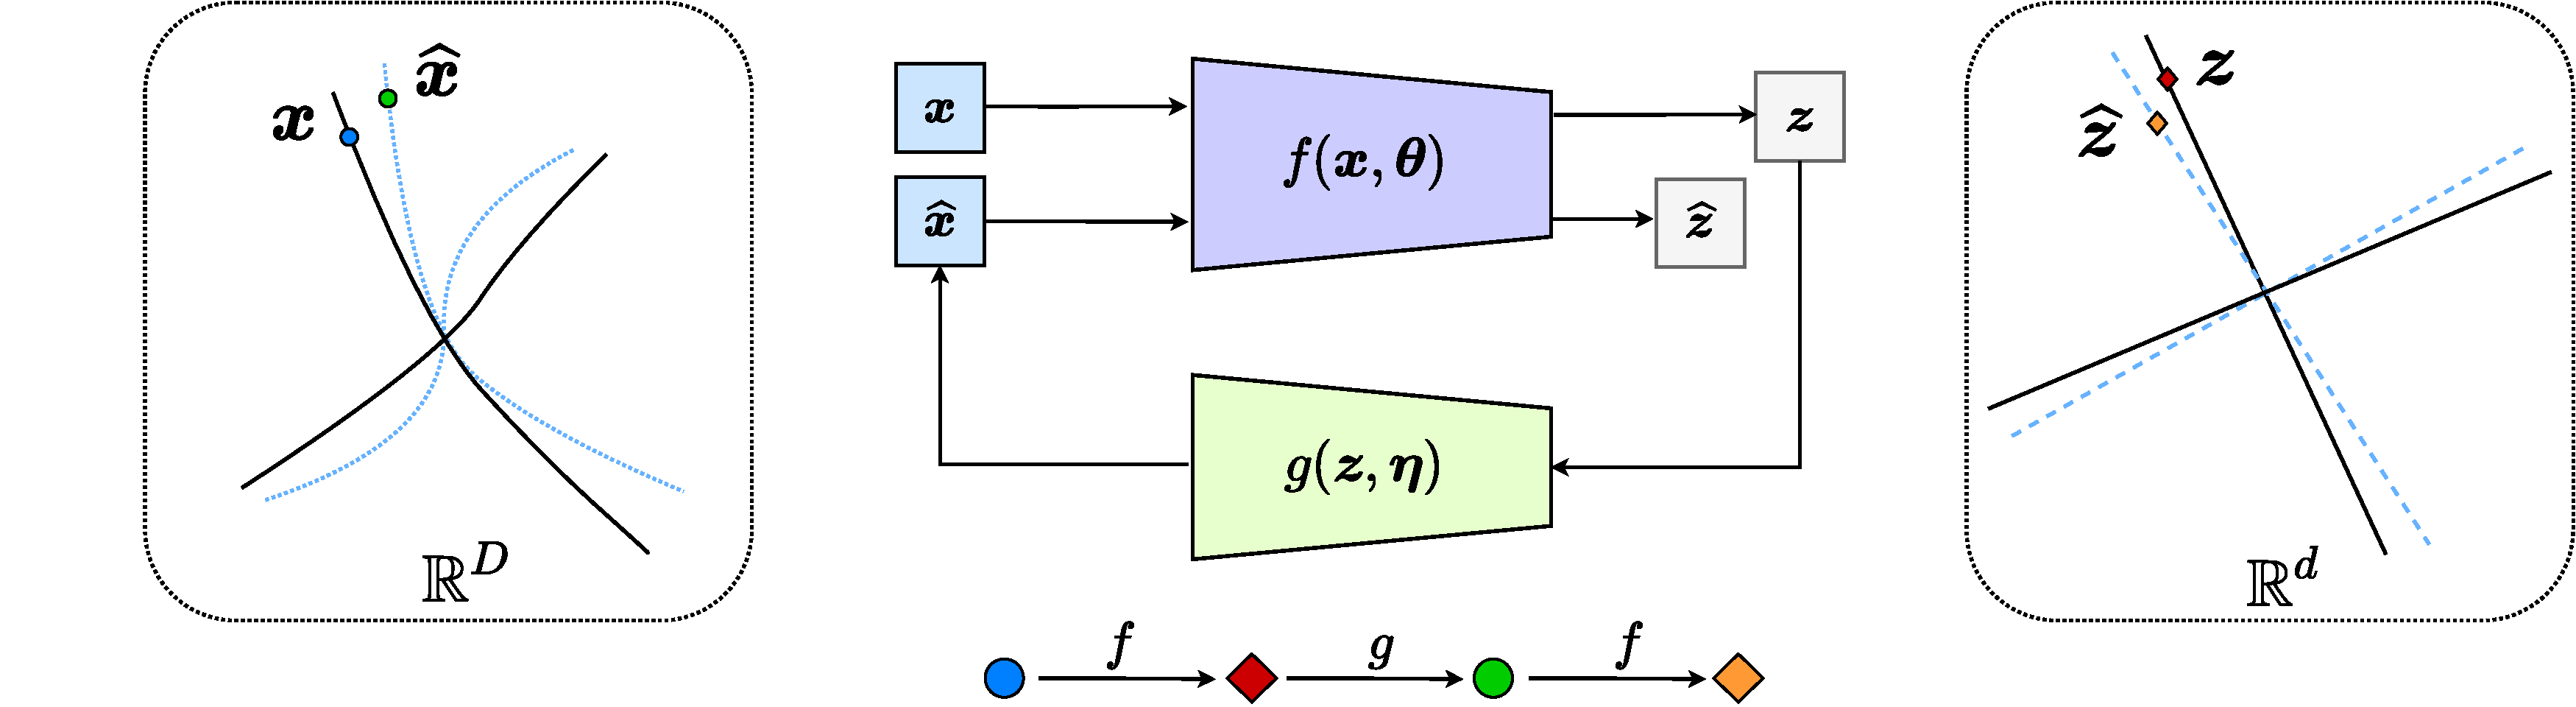
\includegraphics[width=1.0\linewidth]{\toplevelprefix/chapters/chapter5/figs/diagrams_redu_gan_2.pdf}}
\caption{{\bf %Moved after its first citation. Please confirm.
 A Closed-loop Transcription.} The encoder $f$ has dual roles: it learns a representation $\z$ for the data $\x$ via maximizing the rate reduction of $\z$ and it is also a ``feedback sensor'' for any discrepancy between the data $\x$ and the decoded $\hat \x$. The decoder $g$ also has dual roles: it is a ``controller'' that corrects the  discrepancy between $\x$ and $\hat \x$ and it also aims to minimize the overall coding rate for the learned~representation.} \label{fig:auto-encoding-closed} 
\end{figure}


\paragraph{Encoder and decoder as a two-player game.}
Obviously, to ensure the learned auto-encoding to be self-consistent,  the main goal of the decoder $g(\cdot, \bm \eta)$ is to {\em minimize} the distance between $\Z$ and $\hat \Z$. That is, to learn $g$, we want to minimize the distance $d(\Z, \hat \Z)$:
\begin{equation}
\min_g d(\Z, \hat \Z) \doteq \min_\eta  \sum_{k=1}^K \Delta R\big(\Z_k, \hat{\Z}_k\big) =  \min_{\bm \eta}  \sum_{k=1}^K \Delta R\big(\Z_k, f(g(\Z_k, \bm \eta),\bm \theta)\big),
\label{eqn:min-distance}
\end{equation}
where $\Z_k = f(\X_j,\bm \theta)$ and $\hat \Z_k = f(\hat{\X}_k,\bm\theta)$. 

\begin{example}
One may wonder why we need the mapping $f(\cdot, \bm \theta)$ to function as a discriminator between $\X$ and $\hat \X$ by maximizing $\max_{\bm \theta} \Delta R\big(f(\X,\bm \theta), f(\hat \X, \bm \theta)\big)$. Figure~\ref{fig:decoder} gives a simple illustration: there might be many decoders $g$ such that $f\circ g$ is an identity (Id) mapping. $f\circ g(\z) = \z $ for all $\z$ in the subspace $S_{\z}$ in the feature space. However, $g\circ f$ is not necessarily an auto-encoding map for $\x$ in the original distribution $S_{\x}$ (here for simplicity drawn as a subspace). That is, $g\circ f(S_{\x}) \not\subset S_{\x}$, let alone $g\circ f(S_{\x}) = S_{\x}$ or $g\circ f(\x) = \x$. One should expect, without~careful control of the image of $g$, with~high probability, this would be the case, especially when the support of the distribution of $\x$ is extremely  low-dimensional in the original high-dimensional data space. 
\end{example}
\begin{figure}
%\vspace{-1mm}
\centering{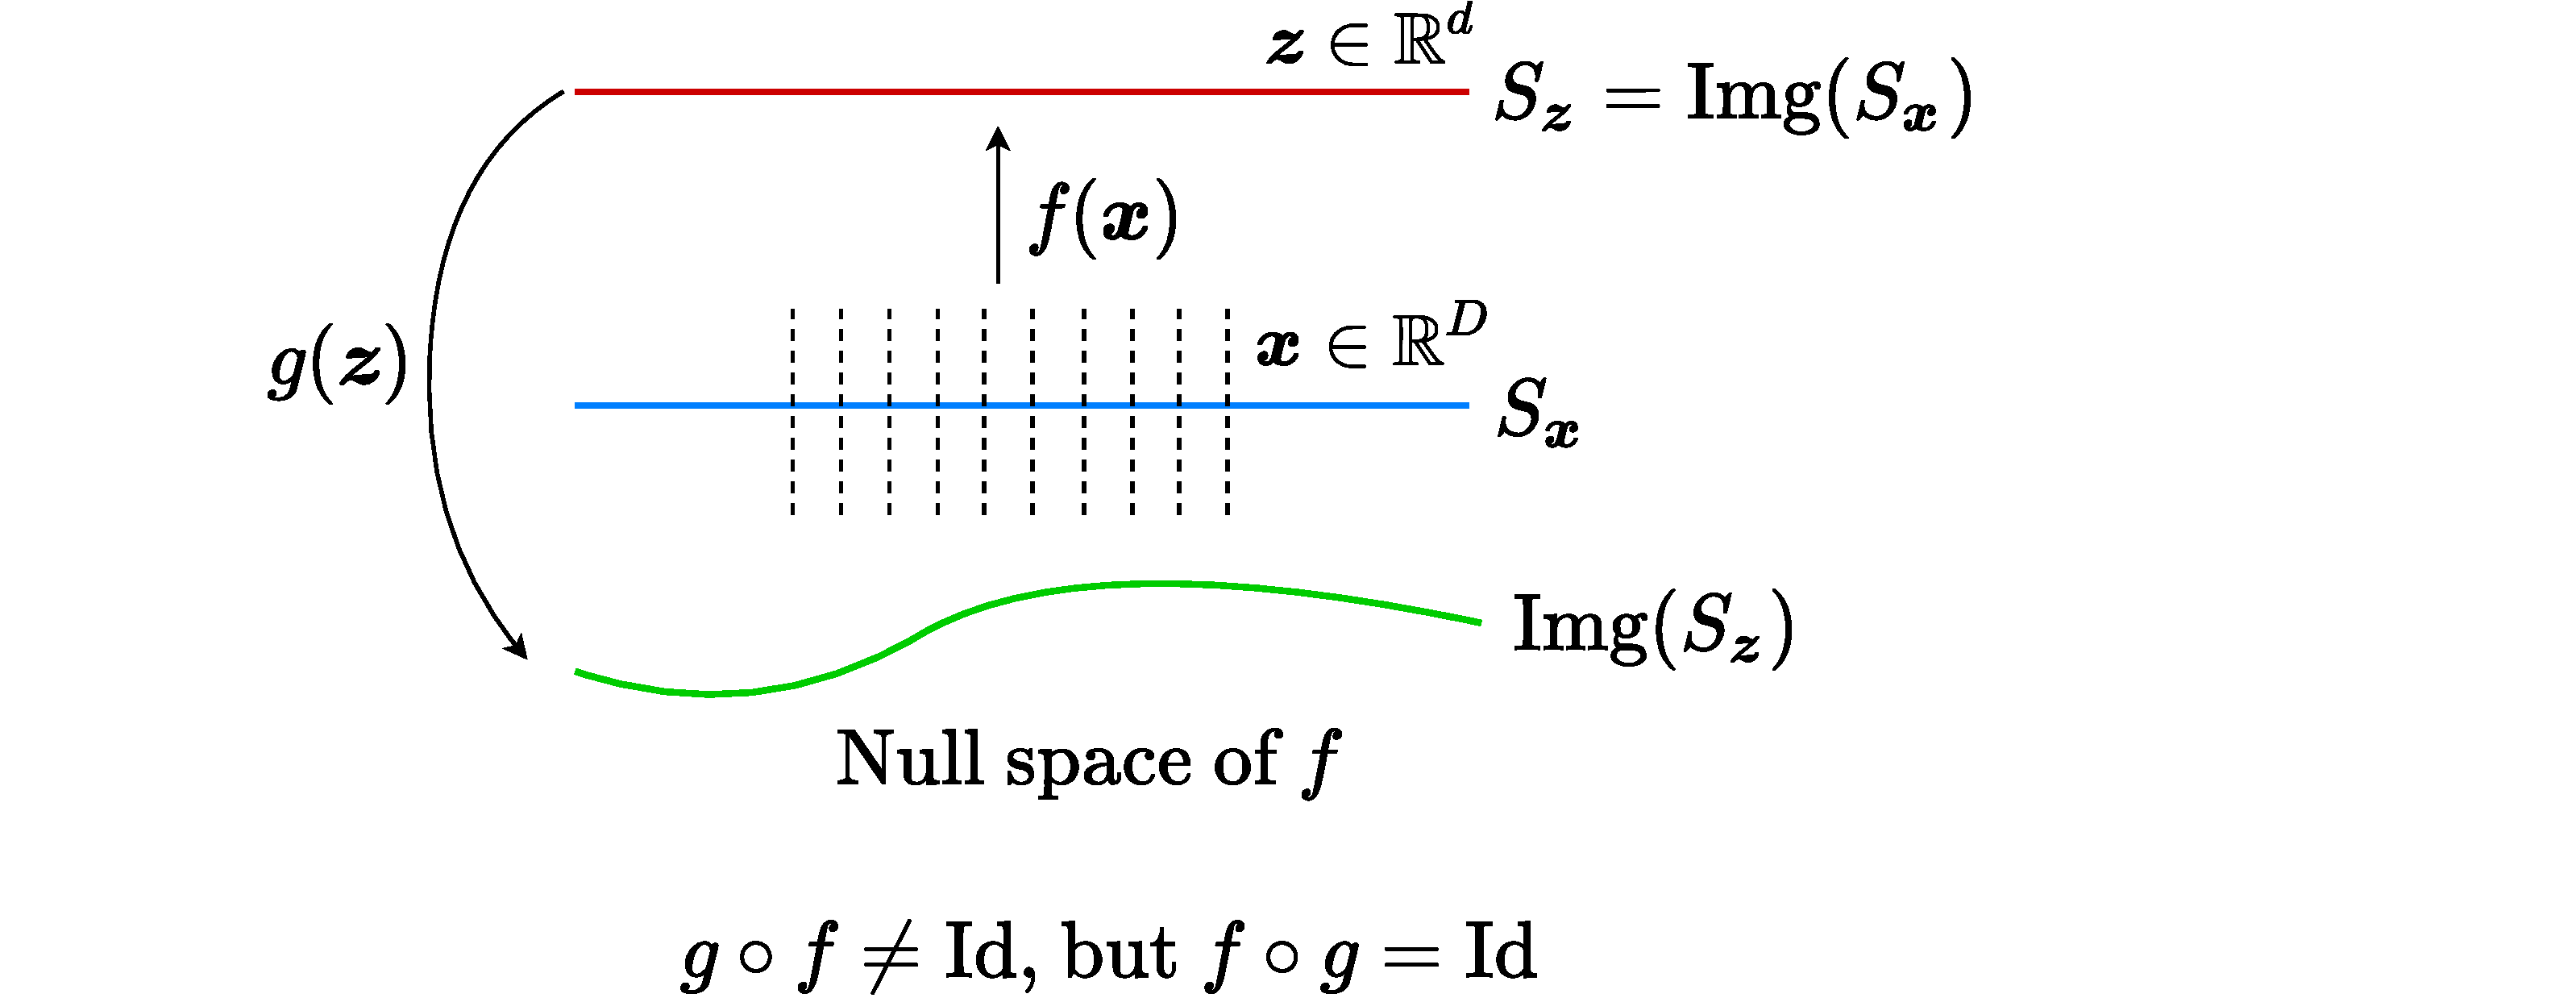
\includegraphics[width=3.0in]{\toplevelprefix/chapters/chapter5/figs/diagrams_fig1.pdf}}
\caption{\textbf{{Embeddings} %Moved after first citation. Please confirm.
 of low-dim submanifolds in a high-dim space.} $S_{\x}$ (blue) is the submanifold for the original data $\x$; $S_{\z}$ (red) is the image of $S_{\x}$ under the mapping $f$, representing the learned feature $\z$; and the green curve  is the image of the feature $\z$ under the decoding \mbox{mapping $g$.} } \label{fig:decoder}
\end{figure} 

Comparing the contractive and contrastive nature of \eqref{eqn:min-distance} and \eqref{eqn:max-distance} on the same distance measure, we see the roles of the encoder $f(\cdot, \bm \theta)$ and the decoder $g(\cdot, \bm \eta)$ naturally as ``{\bf a  two-player game}'': {\em while the encoder $f$ tries to magnify the difference between the original data and their transcribed data, the decoder $g$ aims to minimize the difference.} Now for convenience, let us define the ``closed-loop encoding'' function:
\begin{equation}
    h(\x, \bm \theta,\bm \eta) \doteq f\big(g\big(f(\x, \bm \theta), \bm \eta\big), \bm \theta\big): \; \x \mapsto \hat \z.
\end{equation}

Ideally, we want this function to be very close to $f(\x, \bm \theta)$ or at least the distributions of their images should be close. With~this notation, combining \eqref{eqn:min-distance} and \eqref{eqn:max-distance}, a~closed-loop notion of ``distance'' between $\X$ and $\hat \X$ can be computed as {\em an equilibrium point} to the following Stackelberg game (cf \Cref{sec:minimax}) for the same utility in terms of rate reduction:% (theoretically, there might be significant difference in formulating and seeking the desired solution as the equilibrium point to a min-max or max-min game. In~practice, we do not see major differences as we optimize the program by simply alternating between minimization and maximization. We leave a more careful investigation to future work):
\begin{equation}
\mathcal{D}(\X, \hat \X) \doteq  \max_{\bm \theta} \min_{\bm \eta} \sum_{k=1}^K \Delta R\big(f(\X_k,\bm \theta), h(\X_k,\bm \theta,\bm \eta)\big).
    \label{eq:MCR2-GAN-pair}
\end{equation}

Notice that this only measures the difference between (features of) the original data and its transcribed version. It does not measure how good the representation $\Z$ (or $\hat \Z$) is for the multiple classes within $\X$ (or $\hat \X$). To~this end, we may combine the above distance with the original MCR$^2$-type objectives  \eqref{eq:mcr2-formulation}: namely, the~rate reduction $\Delta R(\Z)$ and $\Delta R(\hat \Z)$ for the learned LDR $\Z$ for $\X$ and $\hat \Z$ for the decoded $\hat \X$. Notice that although the encoder $f$ tries to {\em maximize} the multi-class rate reduction of the features $\Z$ of the data $\X$,  the decoder $g$ should {\em minimize} the rate reduction of the multi-class  features $\hat \Z$ of the decoded $\hat \X$. That is, the decoder $g$ tries to use a minimal  coding rate needed to achieve a good decoding~quality. 

Hence, the~overall ``multi-class''  Stackelberg game for learning the closed-loop transcription, named CTRL-Multi, is
\begin{eqnarray}
&&\max_{\bm \theta} \min_{\bm \eta} \mathcal{T}_{\X}(\bm \theta, \bm \eta) \\
&\doteq& \underbrace{\Delta R\big(f(\X,\bm \theta)\big)}_{\text{Expansive encode}} + \underbrace{\Delta R\big(h(\X,\bm \theta, \bm \eta)\big)}_{\text{Compressive decode}} + \sum_{k=1}^K \underbrace{\Delta R\big(f(\X_j,\bm \theta), h(\X_j,\bm \theta,\bm \eta)\big)}_{\text{Contrastive encode \& Contractive decode}} \nonumber \\
&=& \Delta R\big(\Z(\bm \theta) \big) + \Delta R\big(\hat \Z(\bm \theta, \bm \eta)\big) + \sum_{k=1}^K \Delta R\big(\Z_j(
\bm \theta), \hat \Z_j(\bm \theta, \bm \eta) \big),
    \label{eq:MCR2-GAN-objective}
\end{eqnarray}
subject to certain constraints (upper or lower bounds) on the first term and the second term.  %Such constrained minimax games have also started to draw attention lately \cite{dai2020optimality}. %Please ensure meaning is retained in this paragraph

% \begin{adjustwidth}{-\extralength}{0cm}
% \centering %% If there is a figure in wide page, please release command \centering

% \end{adjustwidth}

Notice that, without~the terms associated with the generative part $h$ or with all such terms fixed as constant, the~above objective is precisely the original MCR$^2$ objective introduced in Chapter \ref{ch:compression}. In an unsupervised setting, if~we view each sample (and its augmentations) as its own class, the~above formulation remains exactly the same. The number of classes $k$ is simply the number of independent samples. In addition, notice that the above game's objective function depends only on (features of) the data $\X$, hence one can learn the encoder and decoder (parameters) without the need for sampling or matching any additional distribution (as typically needed in GANs or VAEs).

As a special case, if~$\X$ only has one class, the Stackelberg game reduces to a special ``two-class'' or ``binary''  form,\footnote{as the first two rate reduction terms automatically become zero} named CTRL-Binary, 
\begin{equation}
 \max_{\bm \theta} \min_{\bm \eta} \mathcal{T}^b_{\X}(\bm \theta, \bm \eta) \doteq \Delta R\big(f(\X,\bm \theta), h(\X,\bm \theta,\bm \eta)\big) = \Delta R\big(\Z(\bm \theta), \hat \Z(\bm \theta, \bm \eta)\big), 
    \label{eq:MCR2-GAN-objective-binary}
\end{equation}
between~$\X$ and the decoded $\hat\X$ by viewing $\X$ and $\hat \X$ as two classes $\{\bm 0, \bm 1\}$. Notice that this binary case resembles the formulation of the original GAN \eqref{eqn:GAN}. Instead of using cross entropy, our formulation adopts a more refined rate-reduction measure, which has been shown to promote diversity in the learned representation in Chapter \ref{ch:compression}. %Please ensure meaning is retained

Sometimes, even when $\X$ contains multiple classes/modes, one could still view all classes together as one class. Then, the above binary objective is to align the union distribution of all classes with their decoded $\hat \X$. This is typically a simpler task to achieve than the multi-class one \eqref{eq:MCR2-GAN-objective}, since it does not require learning of a more refined multi-class CTRL for the data, as~we will later see in experiments. Notice that one good characteristic of the above formulation is that {\em all quantities in the objectives are measured in terms of rate reduction for the learned features} (assuming features eventually become subspace Gaussians). 

One may notice that the above learning framework draws inspiration from closed-loop error correction widely practiced in feedback control systems. The closed-loop mechanism is used to form an overall feedback system between the two encoding and decoding networks for correcting any  ``error'' in the distributions between the data $\x$ and the decoded $\hat \x$. Using terminology from control theory, one may view the encoding network $f$ as a ``sensor'' for error feedback while the decoding network $g$ as a ``controller'' for error correction. However, notice that here the ``target'' for control is not a scalar nor a finite dimensional vector, but~a continuous distribution---in order for the distribution of $\hat \x$ to match that of the data $\x$. This is in general a control problem in an infinite dimensional space. The space of possible diffeomorphisms of submanifolds that $f$ tries to model is infinite-dimensional \cite{Lee2002IntroductionTS}. Ideally, we hope when the sensor $f$ and the controller $g$ are optimal, the distribution of $\x$ becomes a ``fixed point'' for the closed loop while the distribution of $\z$ reaches a compact linear discriminative representation. Hence, the minimax programs \eqref{eq:MCR2-GAN-objective} and \eqref{eq:MCR2-GAN-objective-binary} can also be interpreted as games between an error-feedback sensor and an error-reducing~controller.

The remaining question is whether the above framework can indeed learn a good (autoencoding) presentation of a given dataset? Before we give some formal theoretical justification (in the next subsection), we present some empirical results. 

\paragraph{Visualizing correlation of features $\Z$ and decoded features $\hat \Z$.} We visualize the cosine similarity between $\Z$ and $\hat{\Z}$ learned from the multi-class objective \eqref{eq:MCR2-GAN-objective} on MNIST, CIFAR-10 and ImageNet (10 classes), which indicates how close $\hat{\z} = f\circ g(\z)$ is from $\z$. Results in Figure~\ref{fig:justifyz=z} show that $\Z$ and $\hat{\Z}$ are aligned very well within each class. The~block-diagonal patterns for MNIST are sharper than those for CIFAR-10 and ImageNet, as~images in CIFAR-10 and ImageNet have more diverse visual~appearances.

\begin{figure}[t]
    \begin{subfigure}[t]{0.3\textwidth}
        \centering
        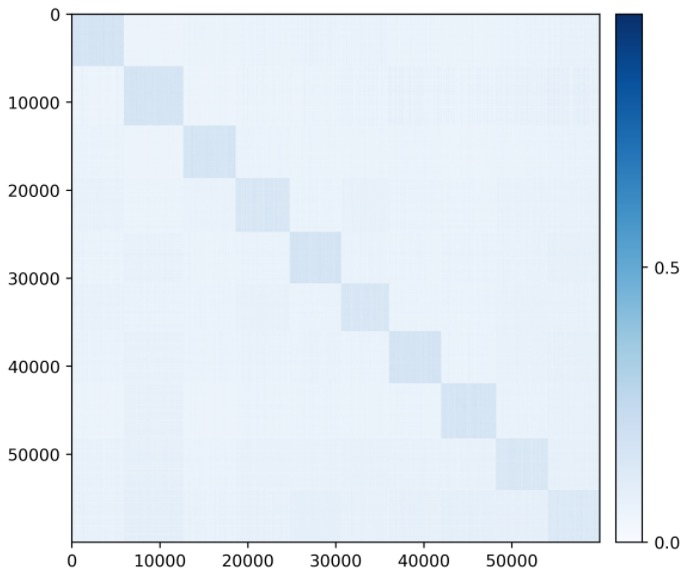
\includegraphics[width=\textwidth]{\toplevelprefix/chapters/chapter5/figs/MNIST_MNIST_ZZhat_heatmap_epo200.png}
        \caption{MNIST}
    \end{subfigure}
    \hfill
    \begin{subfigure}[t]{0.3\textwidth}
        \centering
        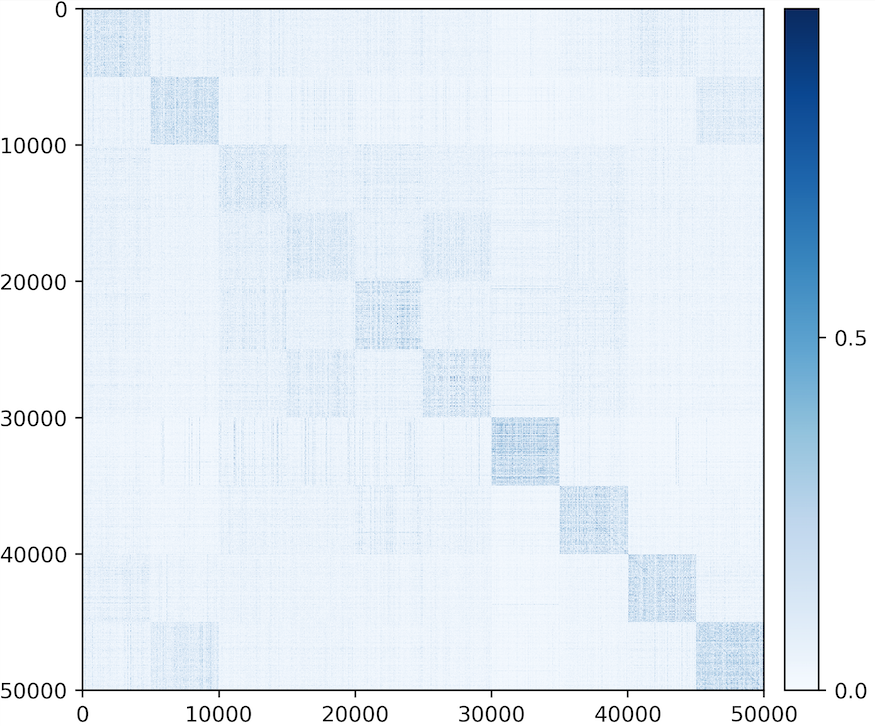
\includegraphics[width=\textwidth]{\toplevelprefix/chapters/chapter5/figs/cifar_heatmat_cifar.png}
        \caption{CIFAR-10}
    \end{subfigure}
    \hfill
    \begin{subfigure}[t]{0.3\textwidth}
        \centering
        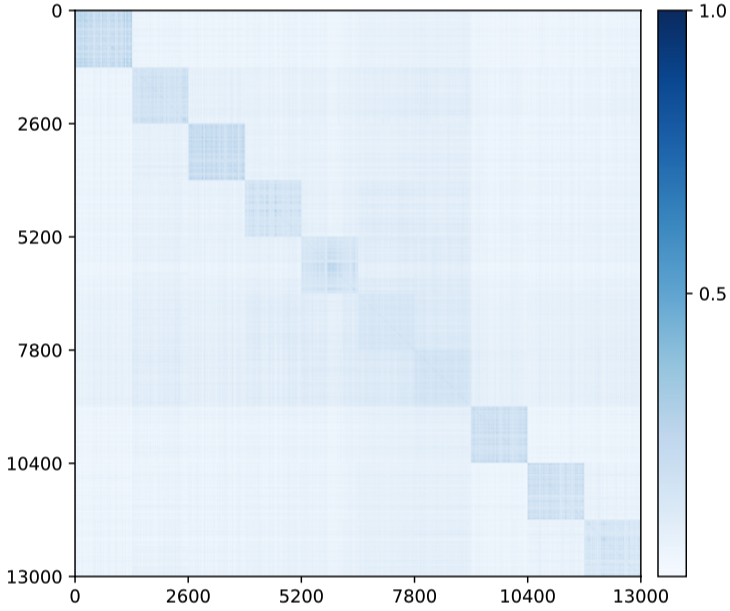
\includegraphics[width=\textwidth]{\toplevelprefix/chapters/chapter5/figs/Imagenet_heatmat_epoch200000.png}
        \caption{ImageNet}
    \end{subfigure}
    \caption{{Visualizing} %Please add comma in five digit numbers in all figures.
    the alignment between $\Z$ and $\hat{\Z}$: $|\Z^\top \hat{\Z}|$ and  in the feature space for (\textbf{a}) MNIST, (\textbf{b}) CIFAR-10, and~(\textbf{c}) ImageNet-10-Class.}
    \label{fig:justifyz=z}
\end{figure}
 


%$\Z$ and $\hat{\Z}$ are the inter-media and output results from CTRL. Both experiments are training and visualizing on train set with Equation~(\ref{eq:MCR2-GAN-objective}). The results show that $\Z$ and $\hat{\Z}$ are aligned well. For the result on MNIST, the diagonal of the matrix is clear compare with the rest part which means the feature space $\Z$ and $\hat{\Z}$ of MNIST can be aligned well by CTRL. CIFAR-10 is a little bit worse than MNIST, but still clear. Even for ImageNet, the diagonal of the matrix is still acceptable. With the more and more complexity of the data, it is reasonable for the decrease of the CTRL alignment ability.



\paragraph{Visualizing auto-encoding of the data $\X$ and the decoded $\hat \X$.} We compare some representative $\X$ and $\hat{\X}$ on MNIST, CIFAR-10 and ImageNet (10 classes) to verify how close $\hat \x = g\circ f(\x)$ is to $\x$. The results are shown in \Cref{fig:justfy_xhat_equals_x}, and visualizations are created from training samples. Visually, the auto-encoded $\hat \x$ faithfully captures major visual features from its respective training sample $\x$, especially the pose, shape, and layout. For the simpler dataset such as MNIST, auto-encoded images are almost identical to the original. %The visual quality is clearly better than other GAN+VAE-type methods, such as  VAE-GAN \citep{VAE-GAN} and BiGAN \citep{donahue2016adversarial}. We refer the reader to Appendices \ref{app:MNIST}, \ref{app:CIFAR} and~\ref{app:imagenet} for more visualization of results on these datasets, including similar results on transformed MNIST digits. More visualization results for learned models on real-life image datasets such as STL-10, CeleB, and~LSUN can be found in the Appendices \ref{app:stl-10} and \ref{app:celeba_lsun}.

%Both experiments are training and visualizing on train set with Equation~(\ref{eq:MCR2-GAN-objective}). The results show that $\X$ and $\hat{\X}$ are aligned which means CTRL has the property to enforce the auto-encoding. One amazing thing is that the CTRL can make exactly one-one mapping on MNIST (compare Figure~\ref{fig:justfy_xhat_equals_x}(a) and Figure~\ref{fig:justfy_xhat_equals_x}(b)).

\begin{figure}[t]
    \begin{subfigure}[t]{0.3\textwidth}
        \centering
        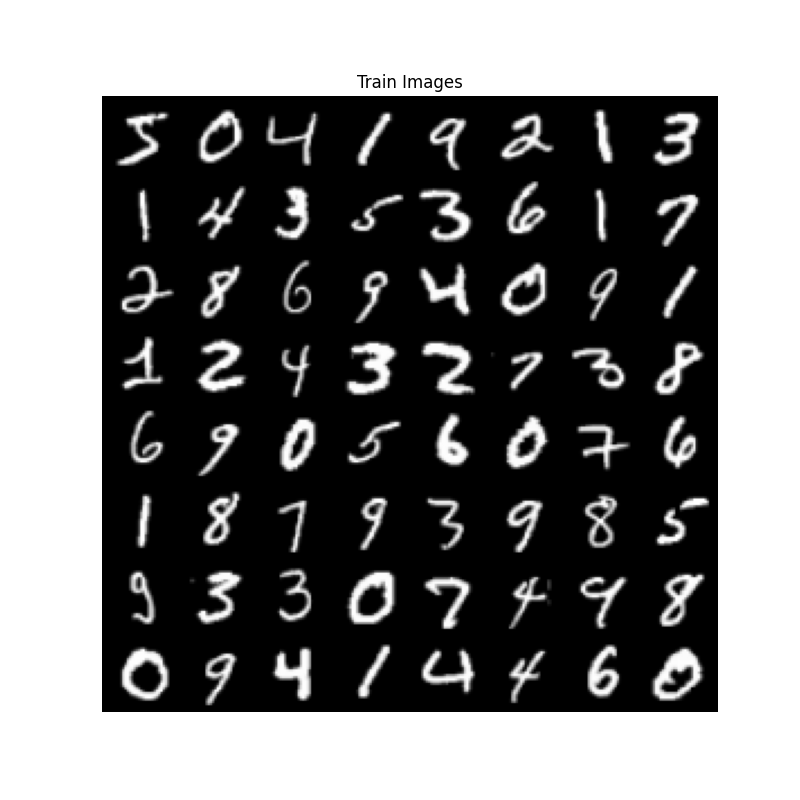
\includegraphics[width=\textwidth]{\toplevelprefix/chapters/chapter5/figs/MNIST_MNIST_train_images_epoch200.png}
        \caption{{\small MNIST $\X$}}
    \end{subfigure}
    \hfill
    \begin{subfigure}[t]{0.3\textwidth}
        \centering
        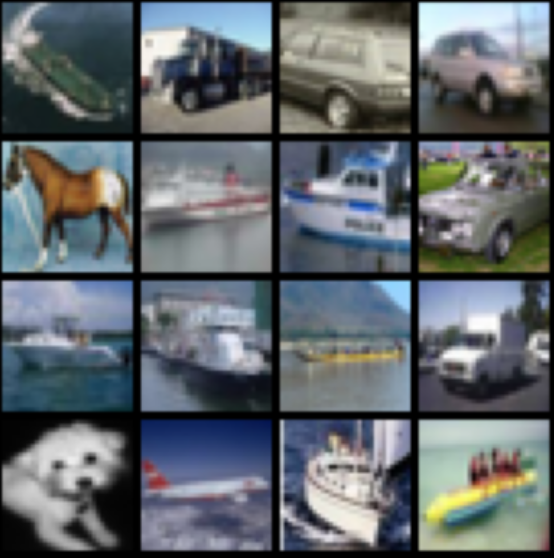
\includegraphics[width=\textwidth]{\toplevelprefix/chapters/chapter5/figs/cifar_input.png}
        \caption{{\small CIFAR-10 $\X$}}
    \end{subfigure}
    \hfill
    \begin{subfigure}[t]{0.3\textwidth}
        \centering
        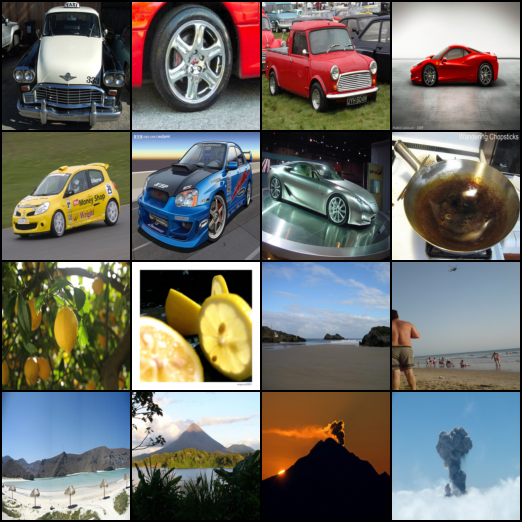
\includegraphics[width=\textwidth]{\toplevelprefix/chapters/chapter5/figs/Imagenet_input.png}
        \caption{{\small ImageNet $\X$}}
    \end{subfigure}

    \begin{subfigure}[t]{0.3\textwidth}
        \centering
        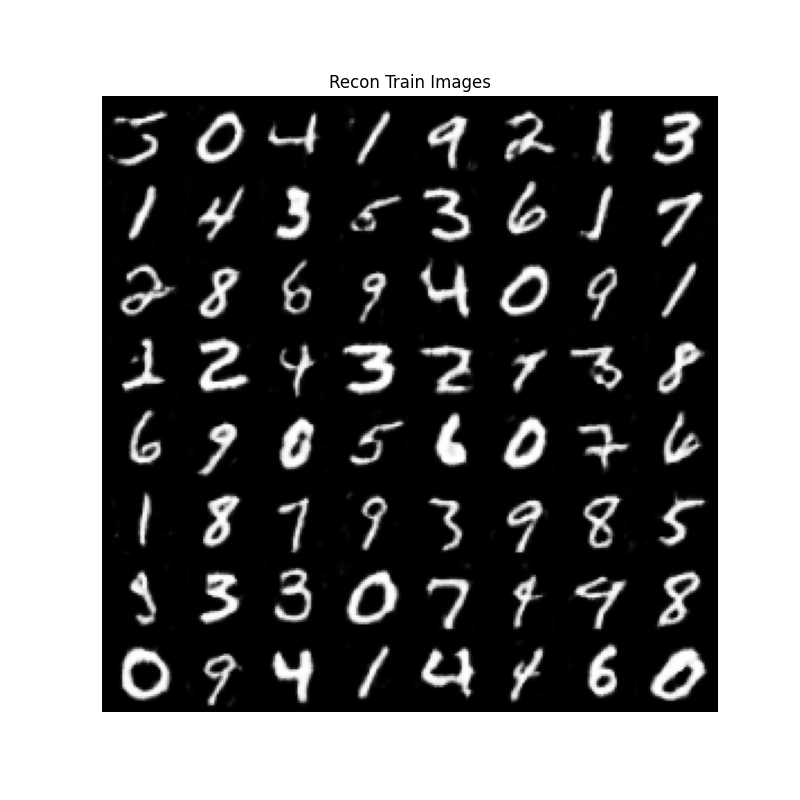
\includegraphics[width=\textwidth]{\toplevelprefix/chapters/chapter5/figs/MNIST_MNIST_train_recon_images_epoch200_multi.png}
        \caption{{\small MNIST $\hat{\X}$}}
    \end{subfigure}
    \hfill
    \begin{subfigure}[t]{0.3\textwidth}
        \centering
        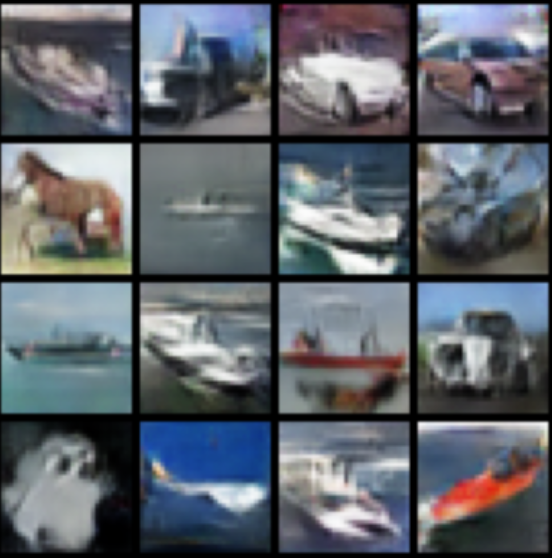
\includegraphics[width=\textwidth]{\toplevelprefix/chapters/chapter5/figs/cifar_reconstruct.png}
        \caption{{\small CIFAR-10 $\hat{\X}$}}
    \end{subfigure}
    \hfill
    \begin{subfigure}[t]{0.3\textwidth}
        \centering
        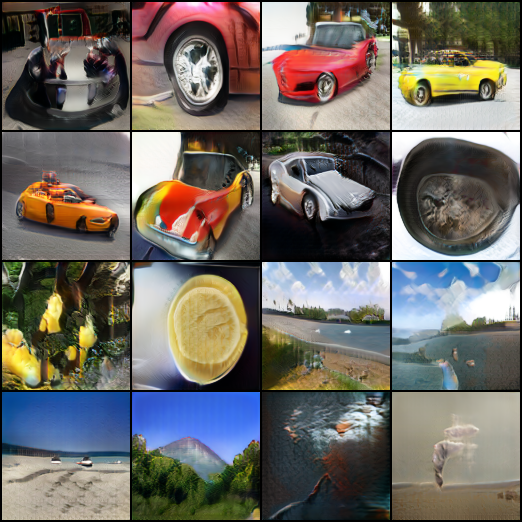
\includegraphics[width=\textwidth]{\toplevelprefix/chapters/chapter5/figs/Imagenet_reconstruct.png}
        \caption{{\small ImageNet $\hat{\X}$}}
    \end{subfigure}
    \caption{Visualizing the auto-encoding property of the learned closed-loop transcription \mbox{($\x \approx \hat{\x} = g\circ f(\x)$)} on MNIST, CIFAR-10, and~ImageNet (zoom in for better visualization).}
<<<<<<< HEAD
    \label{fig:justfy_xhat_equals_x}
=======
    \label{fig:justfy_xhat_equals_x-1}
>>>>>>> overleaf-2025-07-10-0233
\end{figure}
% \begin{figure}
%      \footnotesize
%      %\centering
%      \subfigure[{\small MNIST $\X$}]{
%          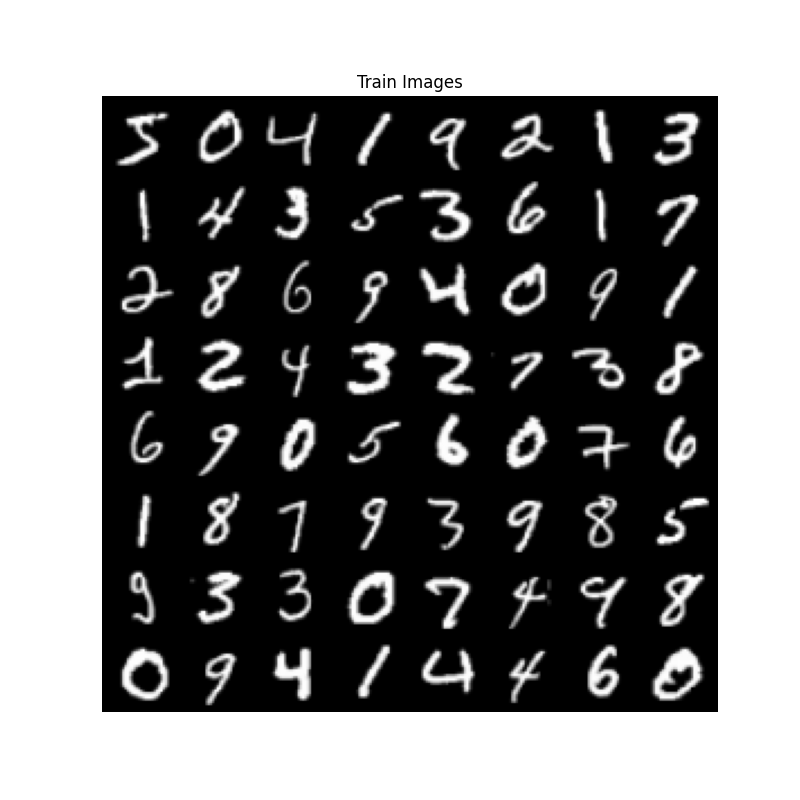
\includegraphics[trim=2.5cm 2cm 2cm 2.5cm ,clip,width=0.3\textwidth]{\toplevelprefix/chapters/chapter5/figs/MNIST_MNIST_train_images_epoch200.png}
%      }   
%      \subfigure[\small CIFAR-10 $\X$]{
%          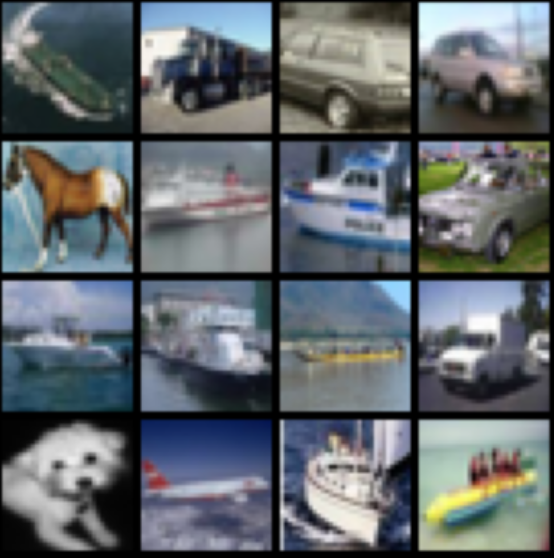
\includegraphics[width=0.3\linewidth]{\toplevelprefix/chapters/chapter5/figs/cifar_input.png}
%      }     
%      \subfigure[\small ImageNet $\X$]{
%          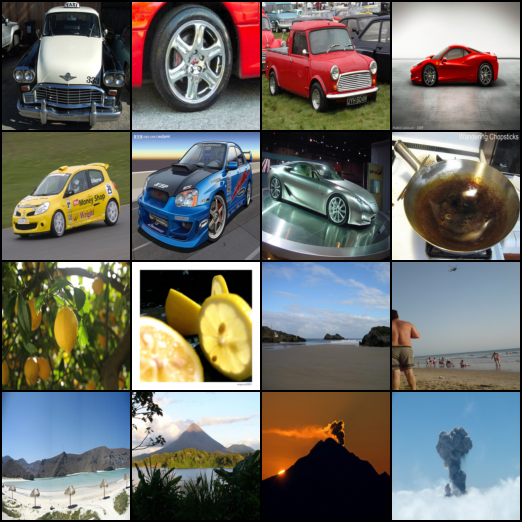
\includegraphics[width=0.3\linewidth]{\toplevelprefix/chapters/chapter5/figs/Imagenet_input.png}
%      }
     
%       \subfigure[\small MNIST $\hat{\X}$]{
%          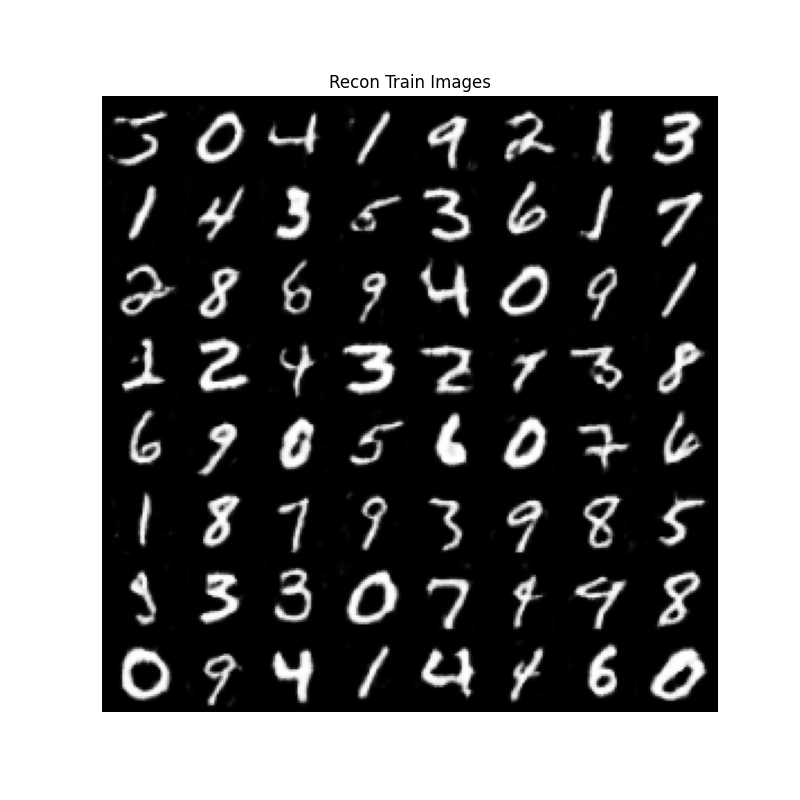
\includegraphics[trim=2.5cm 2cm 2cm 2.5cm ,clip,width=0.3\textwidth]{\toplevelprefix/chapters/chapter5/figs/MNIST_MNIST_train_recon_images_epoch200_multi.png}
%      }
%      \subfigure[\small CIFAR-10 $\hat{\X}$]{
%          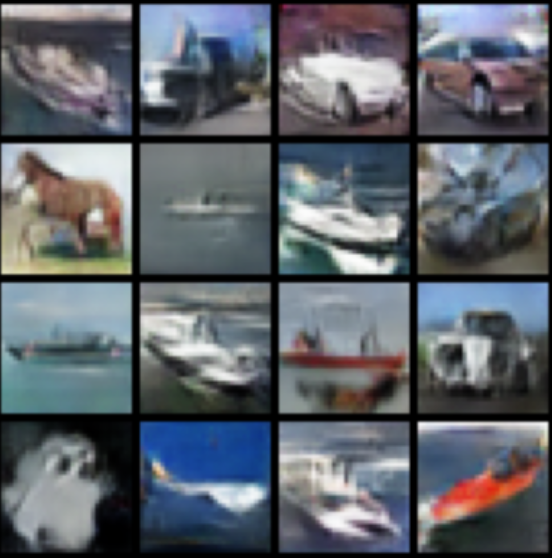
\includegraphics[width=0.3\linewidth]{\toplevelprefix/chapters/chapter5/figs/cifar_reconstruct.png}
%      }
%      \subfigure[\small ImageNet $\hat{\X}$]{
%          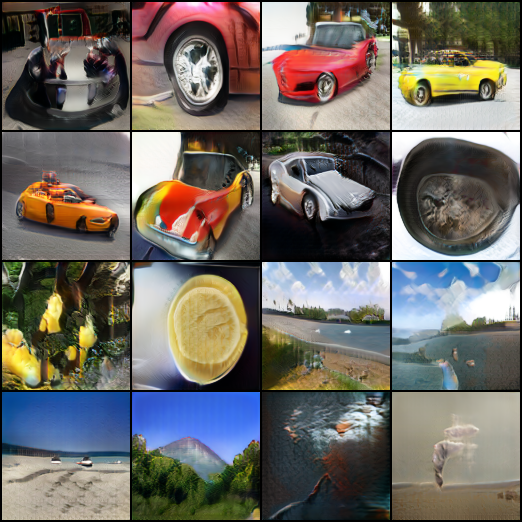
\includegraphics[width=0.3\linewidth]{\toplevelprefix/chapters/chapter5/figs/Imagenet_reconstruct.png}
%     }
%     % \vspace{-0.1in}
%     \caption{Visualizing the auto-encoding property of the learned closed-loop transcription \mbox{($\x \approx \hat{\x} = g\circ f(\x)$)} on MNIST, CIFAR-10, and~ImageNet (zoom in for better visualization).}
%         \label{fig:justfy_xhat_equals_x}
% \end{figure}

\subsection{A Mixture of Low-Dimensional Gaussians}
%This subsection provides theoretical justification for \href{https://arxiv.org/abs/2206.09120}{the ideal case when the distribution of $\X $ is already a mixture of low-dimensional subspaces or low-rank  Gaussians (Druv Pai's work)}.

In the above, we have argued that it is possible to formulate the problem of learning a data distribution as a closed-loop autoencoding problem. We also saw empirically that such a scheme seems to work. The remaining question is when and why such a scheme should works. It is difficult to answer this question for the most general cases with arbitrary data distributions. Nevertheless, as usual, let us see if we can arrive at a rigorous justification for the ideal case when the data distribution is a mixture of low-dimensional subspaces or low-rank Gaussians. A clear characterization and understanding of this important special case would shed light on the more general cases.\footnote{As most distributions with low-dimensional structures can be well-approximated by this family of distributions.}

To this end, let us first suppose that \(\vX\) is distributed according to a mixture of low-dimensional Gaussians, and the label (i.e., subspace assignment) for \(\vX\) is given by \(\vy\). Then, let us set up a minimax optimization problem to learn the data distribution, say through learning an encoding of \(\vX\) into representations \(\vZ\) which are supported on a mixture of \textit{orthogonal} subspaces, and a decoding of \(\vZ\) back into \(\vX\). Then, the representation we want to achieve is maximized by the earlier-discussed version of the information gain, i.e., \( \Delta R_{\epsilon}(\vZ) = R_{\epsilon}(\vZ) - \sum_{k=1}^K R_{\epsilon}(\bm Z_k) \), which enforces that the representation \(\vZ_{k}\) of each class \(k\) spans a subspace which is orthogonal to the supporting subspaces of other classes. The way to measure the consistency of the decoding is, as before, given by \(\sum_{k = 1}^{K}\Delta R(\vZ_{k}, \hat{\vZ}_{k})\), which enforces that the representation \(\vZ_{k}\) and its autoencoding \(\hat{\vZ}_{k}\) for each class \(k\) span the same subspace. Thus, we can set up a simplified Stackelberg game:
\begin{equation}\label{eq:ctrl_msp_game}
    \max_{\bm \theta}\min_{\bm \eta}\bc{\Delta R(\vZ(\bm \theta)) + \sum_{k = 1}^{K}\Delta R(\vZ_{k}(\bm \theta), \hat{\vZ}_{k}(\bm \theta, \bm \eta))}
\end{equation}
Notice that this is a simpler setup than what's used in practice --- there's no \(\Delta R(\hat{\vZ})\) term, for instance, and we work in the supervised setting with class labels (although the techniques used to prove the following result are easy to extend to unsupervised formulations). Also, the consistency of the representations is only measured in a distribution-wise sense via \(\Delta R\) (though this may be substituted with a sample-wise distance metric such as the \(\ell^{2}\) norm if desired, and equivalent conclusions may be drawn, \textit{mutatis mutandis}).

Under mild conditions, in order to realize the desired encoder and decoder which realize \(\vZ\) from a data source \(\vX\) that is already distributed according to a mixture of correlated low-dimensional Gaussians, we only require a linear encoder and decoder to disentangle and whiten the Gaussians. We then study this setting in the case where \(\bm \theta\) and \(\bm \eta\) parameterize matrices whose operator norm is constrained. 

We want to understand what kinds of optima are learned in this setting. One suitable solution concept for this kind of game, where the decoder's optimal solution is defined solely with respect to the encoder (and not, in particular, with respect to some other intrinsic property of the decoder), is a \textit{Stackelberg equilibrium} where the decoder follows the encoder. %\DP{Nika Haghtalab (Berkeley game theory professor) believes very strongly that this should not be called a Stackelberg equilibrium, and the concept of sequential equilibrium is well-defined. Actually, I got a bad grade for my final project because of this naming issue...} 
Namely, at such an equilibrium, the decoder should optimize its objective; meanwhile the encoder should optimize its objective, given that whatever it picks, the decoder will pick an optimal response (which may affect the encoder objective). In game-theoretic terms, it is like the decoder goes \textit{second}: it chooses its weights after the encoder, and both the encoder and decoder attempt to optimize their objective in light of this. It is computationally tractable to learn sequential equilibria via gradient methods via \textit{alternating optimization}, where each side uses different learning rates. Detailed exposition of sequential equilibria is beyond the scope of this book and we provide more technical details in Appendix \ref{sec:minimax}. In this setting, we have the following result:
\begin{theorem}[\cite{pai2022pursuit}, Abridged]\label{thm:ctrl_theory}
    Suppose that \(\vX\) is distributed on a mixture of subspaces. Under certain realistic yet technical conditions, it holds that all sequential equilibria of \eqref{eq:ctrl_msp_game} obey:
    \begin{itemize}
        \item The \(\vZ_{k}\) lie on orthogonal subspaces and are isotropic on those subspaces, i.e., maximizing the information gain.
        \item The autoencoding is self-consistent, i.e., the subspaces spanned by \(\vZ_{k}\) and \(\hat{\vZ}_{k}\) are the same for all \(k\).
    \end{itemize}
\end{theorem}
This notion of self-consistency is the most one can expect if there are only geometric assumptions on the data, i.e., there are no statistical assumptions. If we assume that the columns of \(\vX\) is drawn from a low-rank Gaussian mixture model, then analogous versions of this theorem certify that \(\vZ_{k}\) are also low-rank Gaussians whose covariance is isotropic, for instance. %This phenomenon is validated through experiments, see \DP{TODO}.
Essentially, this result validates, via the simple case of Gaussian mixtures on subspaces, that minimax games to optimize the information gain and self-consistency may achieve optimal solutions.






\section{Continuous Learning Self-Consistent Representations}
\label{sec:continuous}

\subsection{Class-wise Incremental Learning}
\label{sec:class-wise-incremental}
%This subsection shows that the closed-loop architecture is applicable to  \href{https://arxiv.org/abs/2202.05411}{class-wise incremental learning} and it alleviates catastrophic forgetting, probably even with white-box backbone networks. 

As we have seen, deep neural networks have demonstrated a great ability to learn representations for hundreds or even thousands of classes of objects, in both discriminative and generative contexts. However, networks typically must be trained offline, with uniformly sampled data from all classes simultaneously. It has been known that when an (open-loop) network is updated to learn new classes without data from the old ones, previously learned knowledge will fall victim to the problem of {\em catastrophic forgetting} \cite{McCloskey1989catastrophic}. This is known in neuroscience as the stability-plasticity dilemma: the challenge of ensuring that a neural system can learn from a new environment while retaining essential knowledge from previous ones \cite{Grossberg1987CompetitiveLF}.

In contrast, natural neural systems (e.g. animal brains) do not seem to suffer from such catastrophic forgetting at all. They are capable of developing new memory of new objects while retaining memory of previously learned objects. This ability, for either natural or artificial neural systems, is often referred to as {\em  incremental learning, continual learning, sequential learning}, or {\em life-long learning}~ \cite{controlled-forgetting}.



While many recent works have highlighted how artificial neural systems can be  trained in more flexible ways, the strongest existing efforts toward answering the stability-plasticity dilemma for artificial neural networks typically require either storing raw exemplars \cite{icarl,chaudhry2019tiny} or providing external mechanisms \cite{EWC}. Raw exemplars, particularly in the case of high-dimensional inputs like images, are costly and difficult to scale, while external mechanisms --- which typically include secondary networks and representation spaces for generative replay, incremental allocation of network resources, network duplication, or explicit isolation of used and unused parts of the network --- require heuristics and incur hidden costs.


Here we are interested in an incremental learning setting that is similar to nature. It  counters these existing practices with two key qualities. 
\begin{enumerate}
    \item The first is that it should be \emph{memory-based.} When learning new classes, no raw exemplars of old classes are available to train the network together with new data. This implies that one has to rely on a compact and thus structured ``memory'' learned for old classes, such as incrementally learned generative representations of the old classes, as well as the associated encoding and decoding mappings~\cite{fearnet}. 
    \item The second is that it should be \emph{self-contained.} Incremental learning takes place in a single neural system with a fixed capacity, and in a common representation space. The ability to minimize forgetting is implied by optimizing an overall learning objective, without external networks, architectural modifications, or resource allocation mechanisms.
\end{enumerate}

The incoherent linear structures for features of different classes closely resemble how objects are encoded in different areas of the inferotemporal cortex of animal brains \cite{Chang-Cell-2017,Bao2020AMO}. The closed-loop transcription $\X \rightarrow \Z \rightarrow \hat{\X} \rightarrow \hat{\Z}$ also resembles popularly hypothesized mechanisms for memory formation \cite{2020Vandeven,Josselyn2020MemoryER}. This leads to a question: since memory in the brains is formed in an incremental fashion, can the above closed-loop transcription framework also support incremental learning?

\paragraph{LDR memory sampling and replay.} The simple linear {\em structures} of LDR make it uniquely suited for incremental learning: the distribution of features $\Z_j$ of each previously learned class can be explicitly and concisely represented by a principal subspace $\mathcal{S}_j$ in the feature space. To preserve the memory of an old class $j$, we only need to preserve the subspace while learning new classes. To this end, we simply sample $m$ representative prototype features on the subspace along its top $r$ principal components, and denote these features as $\Z_{j,old}$. Because of the simple linear structures of LDR, we can sample from $\Z_{j,old}$ by calculating the mean and covariance of $\Z_{j,old}$ after learning class $j$. The storage required is extremely small, since we only need to store means and covariances, which are sampled from as needed. Suppose a total of $t$ old classes have been learned so far. If prototype features, denoted $\Z_{old} \doteq [\Z^1_{old},\ldots, \Z^t_{old}]$, for all of these classes can be preserved when learning new classes, the subspaces $\{\mathcal{S}_j\}_{j=1}^t$ representing past memory will be preserved as well. Details about sampling and calculating mean and convariance can be found in the work of \cite{tong2023incremental}.
%Appendix \ref{algorithm:prototype} and Appendix~\ref{algorithm:Sampling}

\begin{figure*}[t]
\centering
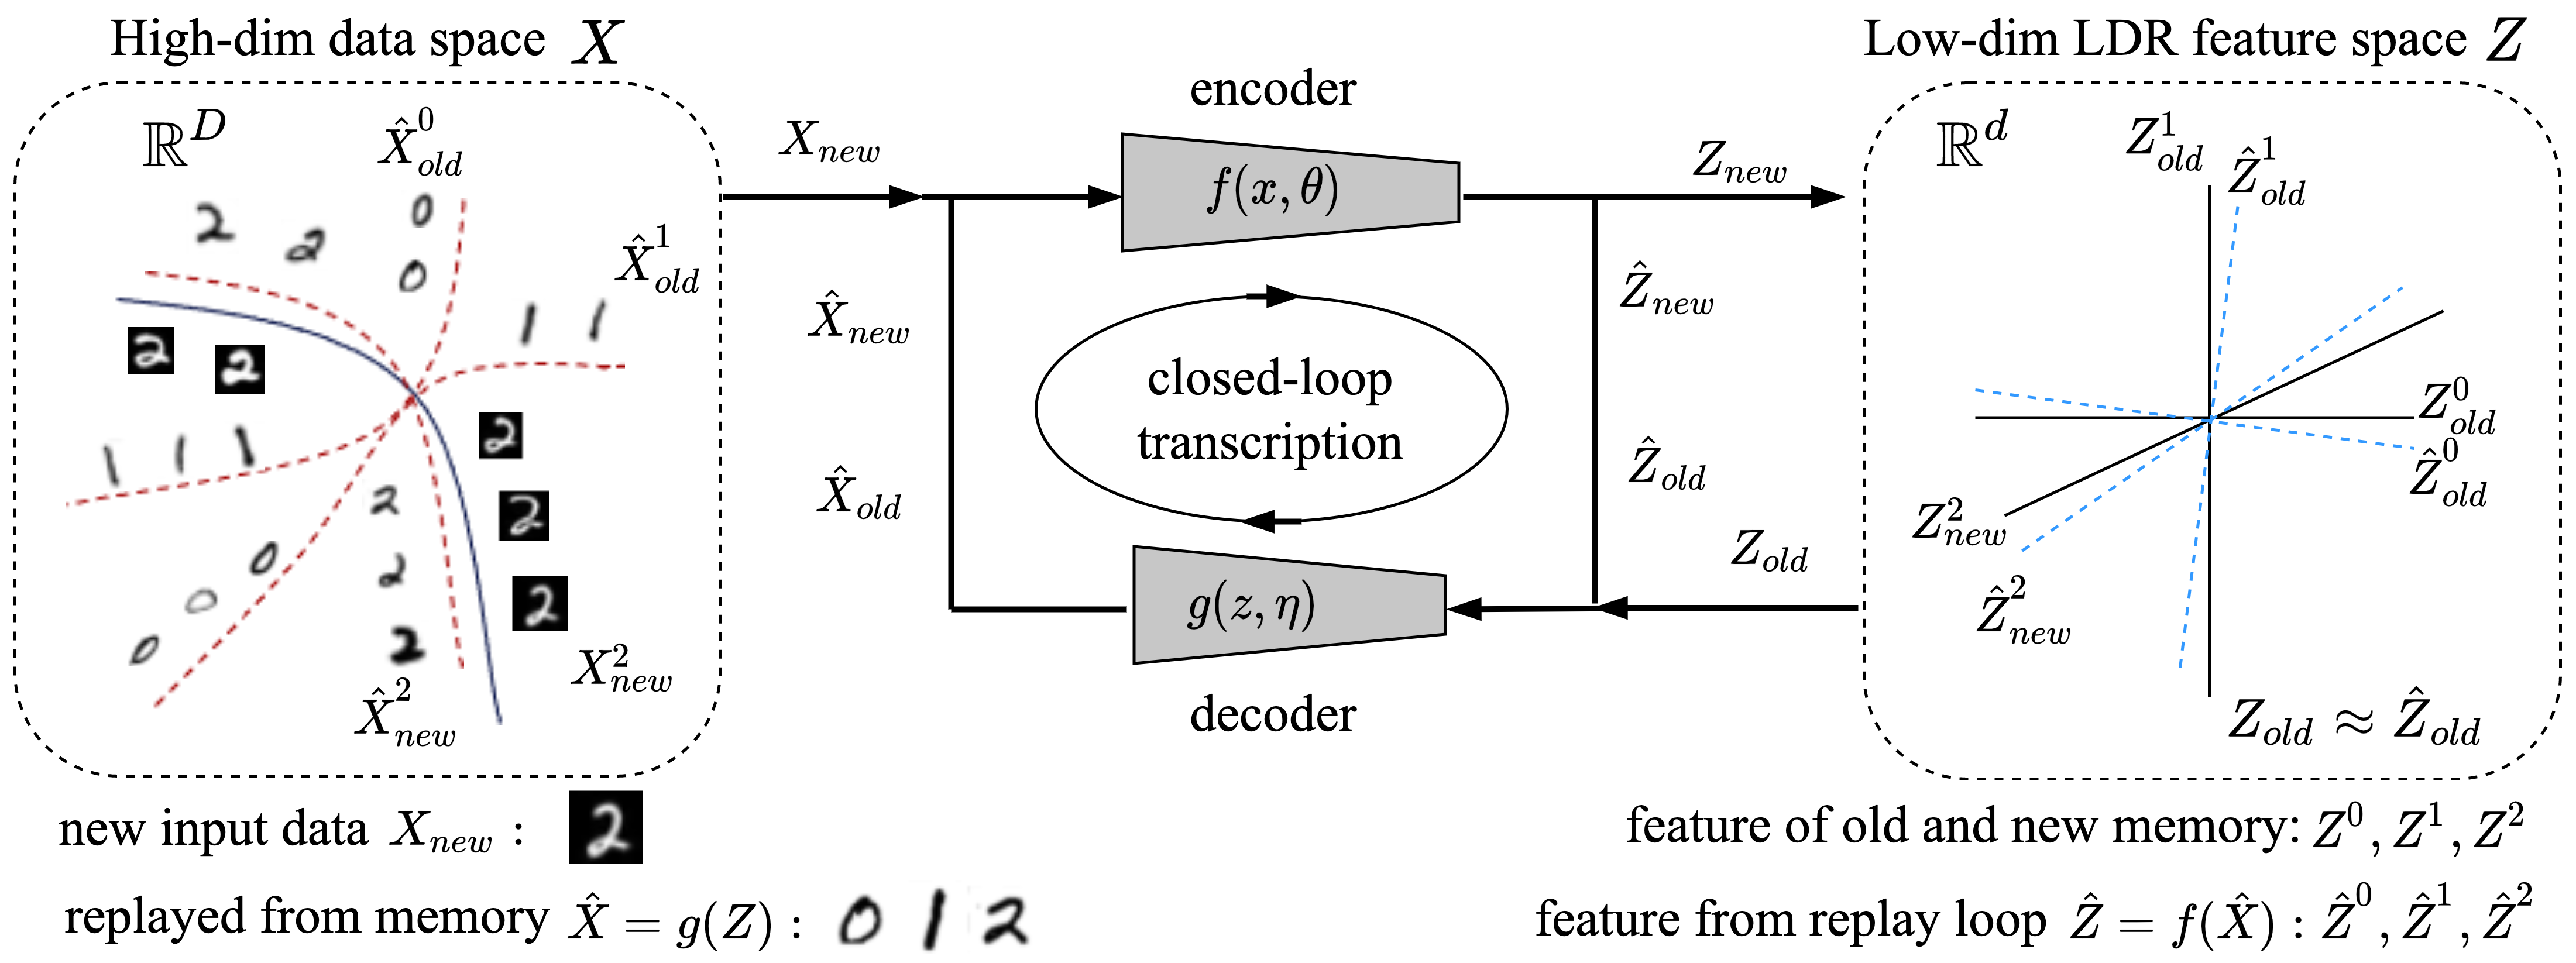
\includegraphics[width=0.9\textwidth]{\toplevelprefix/chapters/chapter5/figs/framework-v7.png}
\caption{\textbf{Overall framework} of our closed-loop transcription based incremental learning for a structured LDR memory. Only a single, entirely self-contained, encoding-decoding network is needed:  for a new data class $\X_{new}$, a new LDR memory $\Z_{new}$ is incrementally learned as a minimax game between the encoder and decoder subject to the constraint that old memory of past classes $\Z_{old}$ is intact through the closed-loop transcription (or replay): $\Z_{old} \approx \hat{\Z}_{old} = f(g(\Z_{old}))$.
\vspace{-0.2in}}
\label{fig:framework}
\end{figure*}

\paragraph{Incremental learning LDR with an old-memory constraint.} 
Notice that, with the learned auto-encoding \eqref{eqn:autoencoding-ch6}, one can replay and use the images, say $\hat\X_{old} = g(\Z_{old}, \eta)$, associated with the memory features  to avoid forgetting while learning new classes. This is typically how generative models have been used for prior incremental learning methods. However, with the closed-loop framework, explicitly replaying images from the features is not necessary. Past memory can be effectively preserved through optimization exclusively on the features themselves.

Consider the task of incrementally learning a new class of objects.\footnote{Of course, one may also consider the more general setting where the task contains a small batch of new classes, without serious modification.} We denote a corresponding new sample set as $\X_{new}$. The features of $\X_{new}$ are denoted as  $\Z_{new}(\theta) = f(\X_{new}, \theta)$. We concatenate them together with the prototype features of the old classes $\Z_{old}$ and form $\Z = [\Z_{new}(\theta), \Z_{old}]$. We denote the replayed images from all features as $\hat{\X} = [{\hat{\X}_{new}(\theta,\eta)}, {\hat{\X}_{old}(\eta)}]$ although we do not actually need to compute or use them explicitly. We only need features of replayed images, denoted $\hat{\Z} = f(\hat{\X}, \theta) =  [{\hat{\Z}_{new}(\theta,\eta)}, {\hat{\Z}_{old}(\theta,\eta)}]$. 


Mirroring the motivation for the multi-class CTRL objective \eqref{eq:MCR2-GAN-objective}, we would like the features of the new class $\Z_{new}$ to be incoherent to all of the old ones $\Z_{old}$. As $\Z_{new}$ is the only new class whose features needs to be learned, the objective \eqref{eq:MCR2-GAN-objective} reduces to the case where $k=1$:
\begin{equation}
\min_\eta \max_\theta \Delta{R(\Z)}+\Delta{R(\hat{\Z})}+\Delta{R(\Z_{new},\hat{\Z}_{new})}.
\label{eqn:unconstrained-minimax}
% \vspace{-2mm}
\end{equation}
However, when we update the network parameters $(\theta, \eta)$ to optimize the features for the new class, the updated mappings $f$ and $g$ will change features of the old classes too. Hence, to minimize the distortion of the old class representations, we can try to enforce $\mbox{Cov}(\Z_{j,old}) = \mbox{Cov}(\hat{\Z}_{j,old})$. In other words, while learning new classes, we enforce the memory of old classes remain ``self-consistent'' through the transcription loop:
\begin{equation}
\Z_{old} \xrightarrow{\hspace{2mm} g(\z,\eta) \hspace{2mm}} \hat \X_{old} \xrightarrow{\hspace{2mm} f(\x, \theta)\hspace{2mm}} \ \hat \Z_{old}.
\end{equation}
Mathematically, this is equivalent to setting 
$$\Delta R(\Z_{old},\hat{\Z}_{old}) \doteq  \sum_{j=1}^t \Delta R(\Z_{j,old},\hat{\Z}_{j,old}) = 0.$$  
Hence, the above minimax program \eqref{eqn:unconstrained-minimax} is revised as a {\em constrained} minimax game, which we refer to as  {\em incremental closed-loop transcription} (i-CTRL).
The objective of this game is identical to the standard multi-class CTRL objective \eqref{eq:MCR2-GAN-objective}, but includes just one additional constraint:
%\begin{small}
\begin{eqnarray}
\min_\eta \max_\theta  &&\Delta{R(\Z)}+\Delta{R(\hat{\Z})}+\Delta{R(\Z_{new},\hat{\Z}_{new})} \nonumber\\
&& \mbox{subject to} \quad  \Delta R(\Z_{old},\hat{\Z}_{old}) = 0.
\label{eqn:constrained-minimax}
\end{eqnarray}
%\end{small}
% This is equivalent to the multi-class CTRL objective \eqref{eq:MCR2-GAN-objective} with an additional constraint $\Delta R(\Z_{old},\hat{\Z}_{old}) = 0$. % is the only thing that we need to modify the original formulation. 

In practice, the constrained minimax program can be solved by {\em alternating}  minimization and maximization between the encoder $f(\cdot, \theta)$ and decoder $g(\cdot, \eta)$ as follows:
%\begin{small}
\begin{eqnarray}
&\max_\theta  &\Delta{R(\Z)}\!+\!\Delta{R(\hat{\Z})}\!+\!\lambda\cdot  \Delta{R(\Z_{new},\hat{\Z}_{new})} - \gamma\cdot \Delta{R(\Z_{old},\hat{\Z}_{old})}, \label{eqn:relaxed-max}\\ 
&\min_\eta &\Delta{R(\Z)}\!+\!\Delta{R(\hat{\Z})}\!+\!\lambda\cdot \Delta{R(\Z_{new},\hat{\Z}_{new})} + \gamma\cdot \Delta{R(\Z_{old},\hat{\Z}_{old})}; \label{eqn:relaxed-min}
\end{eqnarray}
%\end{small}
where the constraint $\Delta R(\Z_{old},\hat{\Z}_{old}) = 0$ in \eqref{eqn:constrained-minimax} has been converted (and relaxed) to a Lagrangian term with a corresponding coefficient $\gamma$ and sign. We additionally introduce another coefficient $\lambda$ for weighting the rate reduction term associated with the new data. % to balance between old and new classes.
%More algorithmic details are given in Appendix \ref{app:algorithm}.



\paragraph{Jointly optimal memory via incremental reviewing.} 
As we will see, the above constrained minimax program can already achieve state of the art performance for incremental learning. Nevertheless, developing an optimal memory for {\em all classes} cannot rely on graceful forgetting alone. Even for humans, if an object class is learned only once, we should expect the learned memory to fade as we continue to learn new others, unless the memory can be consolidated by reviewing old object classes. % repeatedly. 

To emulate this phase of memory forming, after incrementally learning a whole dataset, we may go back to review all classes again, one class at a time. We refer to going through all classes once as one reviewing ``cycle''.\footnote{to distinguish from the term ``epoch'' used in the conventional joint learning setting.} If needed, multiple reviewing cycles can be conducted. It is quite expected that reviewing can improve the learned (LDR) memory. But somewhat surprisingly, the closed-loop framework allows us to review even in a ``{class-unsupervised}'' manner: when reviewing data of an old class say $\X_j$, the system does not need the class label and can simply treat $\X_j$ as a new class $\X_{new}$. That is, the system optimizes the same constrained mini-max program \eqref{eqn:constrained-minimax} without any modification; after the system is optimized, one can identify the newly learned subspace spanned by $\Z_{new}$, and use it to replace or merge with the old subspace $\mathcal{S}_j$. As our experiments show, such an class-unsupervised incremental review process can gradually improve both discriminative and generative performance of the LDR memory, eventually converging to that of a jointly-learned memory.

\paragraph{Experimental verification.}
We show some experimental results on the following datasets: MNIST \cite{lecun1998gradient} and CIFAR-10 \cite{krizhevsky2014cifar}. All experiments are conducted for the more challenging class-IL setting. For both MNIST and CIFAR-10, the 10 classes are split into 5 tasks with 2 classes each or 10 tasks with 1 class each. For the encoder $f$ and decoder $g$, we adopt a very simple network architecture modified from DCGAN \cite{radford2016unsupervised}, which is merely a {\em four-layer} convolutional network. Here we only show some qualitative visual results and more experiments and analytical analysis can be found in the work \cite{tong2023incremental}.

\paragraph{Visualizing auto-encoding properties.}
We begin by qualitatively visualizing some representative images $\X$ and the corresponding replayed $\hat{\X}$ on MNIST and CIFAR-10. The model is learned incrementally with the datasets split into 5 tasks. Results are shown in \Cref{fig:justfy_xhat_equals_x_incremental}, where we observe that the reconstructed $\hat{\X}$ preserves the main visual characteristics of $\X$ including shapes and textures. For a simpler dataset like MNIST, the replayed $\hat{\X}$ are almost identical to the input $\X$! This is rather remarkable given: (1) our method does not explicitly enforce $\hat{\x} \approx \x$ for individual samples as most autoencoding methods do, and (2) after having incrementally learned all classes, the generator has not forgotten how to generate digits learned earlier, such as 0, 1, 2.  For a more complex dataset like CIFAR-10, we also demonstrate good visual quality, faithfully capturing the essence of each image.

\begin{figure}[t]
    \begin{subfigure}[t]{0.20\textwidth}
        \centering
        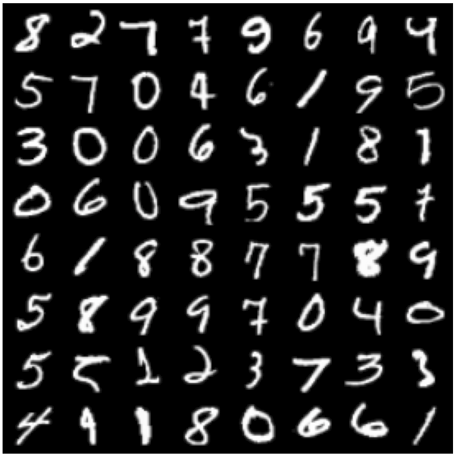
\includegraphics[width=\textwidth]{\toplevelprefix/chapters/chapter5/figs/mnist_x.png}
        \caption{MNIST $\X$}
    \end{subfigure}
    \hfill
    \begin{subfigure}[t]{0.20\textwidth}
        \centering
        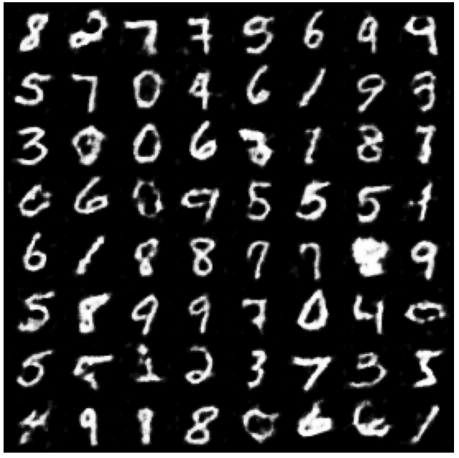
\includegraphics[width=\textwidth]{\toplevelprefix/chapters/chapter5/figs/mnist_recon_x.png}
        \caption{MNIST $\hat{\X}$}
    \end{subfigure}
    \hfill
    \begin{subfigure}[t]{0.20\textwidth}
        \centering
        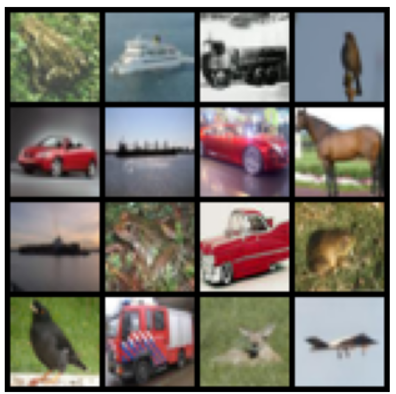
\includegraphics[width=\textwidth]{\toplevelprefix/chapters/chapter5/figs/cifar10_x.png}
        \caption{CIFAR-10 $\X$}
    \end{subfigure}
    \hfill
    \begin{subfigure}[t]{0.20\textwidth}
        \centering
        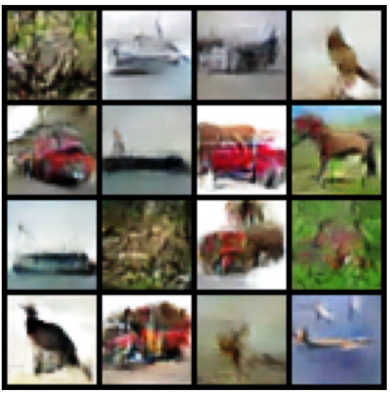
\includegraphics[width=\textwidth]{\toplevelprefix/chapters/chapter5/figs/cifar10_x_recon.png}
        \caption{CIFAR-10 $\hat{\X}$}
    \end{subfigure}
    \caption{\small Visualizing the auto-encoding property of the learned  ($\hat{\X} = g\circ f(\X)$). }
        \label{fig:justfy_xhat_equals_x_incremental}
\end{figure}


\paragraph{Principal subspaces of the learned features.}
Most generative memory-based methods utilize autoencoders, VAEs, or GANs for replay purposes. The structure or distribution of the learned features $\Z_j$ for each class is  unclear in the feature space. The features $\Z_j$ of the LDR memory, on the other hand, have a clear linear structure. Figure \ref{fig:cifar_10_pca_sampling_main} visualizes correlations among all learned features $|\Z^\top\Z|$, in which we observe clear block-diagonal patterns for both datasets.\footnote{Notice that these patterns closely resemble the similarity matrix of response profiles of object categories from different areas of the inferotemporal cortex, as shown in  Extended DataFig.3 of \cite{Bao2020AMO}.} This indicates the features for different classes $\Z_j$ indeed lie on subspaces that are incoherent from one another. Hence, features of each class can be well modeled as a principal subspace in the feature space. %A more precise measure of affinity among those subspaces can be found in Appendix~\ref{app:analysis}.

\begin{figure}[tb]
\centering
\includegraphics[height=4.1cm]{\toplevelprefix/chapters/chapter5/figs/Heatmap_MNIST.jpg}  
\includegraphics[height=4cm]{\toplevelprefix/chapters/chapter5/figs/Heatmap_CIFAR10.png}
\caption{\small Block diagonal structure of $|\Z^\top \Z|$ in the feature space for MNIST (left) and CIFAR-10 (right).}
\label{fig:cifar_10_pca_sampling_main}
\end{figure}

% \begin{figure}[t]
% \centering
%  \subfigure[MNIST]{
%      \includegraphics[width=0.20\textwidth]{Fig/Experiment/MNIST/Heatmap_MNIST.jpg}
%  }
%  \hspace{5mm}
%   \subfigure[CIFAR-10]{
%      \includegraphics[width=0.20\textwidth]{Fig/Experiment/CIFAR10/Heatmap_CIFAR10.png}
%  }
%  \vspace{-0.18in}
%  \caption{\small Block diagonal structure of $|\Z^\top \Z|$ in the feature space for MNIST (left) and CIFAR-10 (right). \vspace{-5mm}}
%  \label{fig:cifar_10_pca_sampling_main}
% \end{figure}


\paragraph{Replay images of samples from principal components.}
Since features of each class can be modeled as a principal subspace, we further visualize the individual principal components within each of those subspaces. Figure \ref{fig:pca_sampling_main} shows the images replayed from sampled features along the top-4 principal components for different classes, on MNIST and CIFAR-10 respectively. Each row represents samples along one principal component and they clearly show similar visual characteristics but distinctively different from those in other rows. We see that the model remembers different poses of `4' after having learned all remaining classes. For CIFAR-10, the incrementally learned memory remembers representative poses and shapes of horses and ships. 

\begin{figure}[t]
    \begin{subfigure}[t]{0.20\textwidth}
        \centering
        \includegraphics[width=\textwidth]{\toplevelprefix/chapters/chapter5/figs/mnist_4.png}
        \caption{sampled $\hat{\x}_{old}$ of `4'}
    \end{subfigure}
    \hfill
    \begin{subfigure}[t]{0.20\textwidth}
        \centering
        \includegraphics[width=\textwidth]{\toplevelprefix/chapters/chapter5/figs/mnist_7.png}
        \caption{sampled $\hat{\x}_{old}$ of `7'}
    \end{subfigure}
    \hfill
    \begin{subfigure}[t]{0.20\textwidth}
        \centering
        \includegraphics[width=\textwidth]{\toplevelprefix/chapters/chapter5/figs/horse_z.jpg}
        \caption{sampled $\hat{\x}_{old}$ of `horse'}
    \end{subfigure}
    \hfill
    \begin{subfigure}[t]{0.20\textwidth}
        \centering
        \includegraphics[width=\textwidth]{\toplevelprefix/chapters/chapter5/figs/ship_z.jpg}
        \caption{sampled $\hat{\x}_{old}$ of `ship'}
    \end{subfigure}
    \caption{\small Visualization of 5 reconstructed $\hat \x=g(\z)$ from $\z$'s with the closest distance to (top-4) principal components of learned features for {MNIST} (class ‘4’ and class ‘7’) and {CIFAR-10} (class ‘horse’ and  ‘ship’).}
    \label{fig:pca_sampling_main}
\end{figure}

% \begin{figure}[t]
% \centering
%  \subfigure[sampled $\hat{\x}_{old}$ of `4']{
%      \includegraphics[width=0.2\textwidth]{chapters/chapter5/figs/mnist_4.png}
%  }
%   \subfigure[sampled $\hat{\x}_{old}$ of `7']{
%      \includegraphics[width=0.2\textwidth]{chapters/chapter5/figs/mnist_7.png}
%  }
%   \subfigure[\footnotesize sampled $\hat{\x}_{old}$ of  `horse']{
%      \includegraphics[width=0.2\textwidth]{chapters/chapter5/figs/horse_z.jpg}
%  }
%   \subfigure[sampled $\hat{\x}_{old}$ of `ship']{
%      \includegraphics[width=0.2\textwidth]{chapters/chapter5/figs/ship_z.jpg}
%  }
%  \caption{\small Visualization of 5 reconstructed $\hat \x=g(\z)$ from $\z$'s with the closest distance to (top-4) principal components of learned features for {MNIST} (class ‘4’ and class ‘7’) and {CIFAR-10} (class ‘horse’ and  ‘ship’).}
%  \label{fig:pca_sampling_main}
% \end{figure}


\paragraph{Effectiveness of incremental reviewing.}
We verify how the incrementally learned LDR memory can be further consolidated with an unsupervised incremental reviewing phase described before. Experiments are conducted on CIFAR-10, with 10 steps. Figure \ref{fig:memory_review} left shows replayed images of the first class `airplane' at the end of incremental learning of all ten classes, sampled along the top-3 principal components -- every two rows (16 images) are along one principal direction. Their  visual quality remains very decent -- observed almost no forgetting. The right figure shows replayed images after reviewing the first class once. We notice a significant improvement in visual quality after the reviewing, and principal components of the features in the subspace start to correspond to distinctively different visual attributes within the same class.

\begin{figure}
\centering
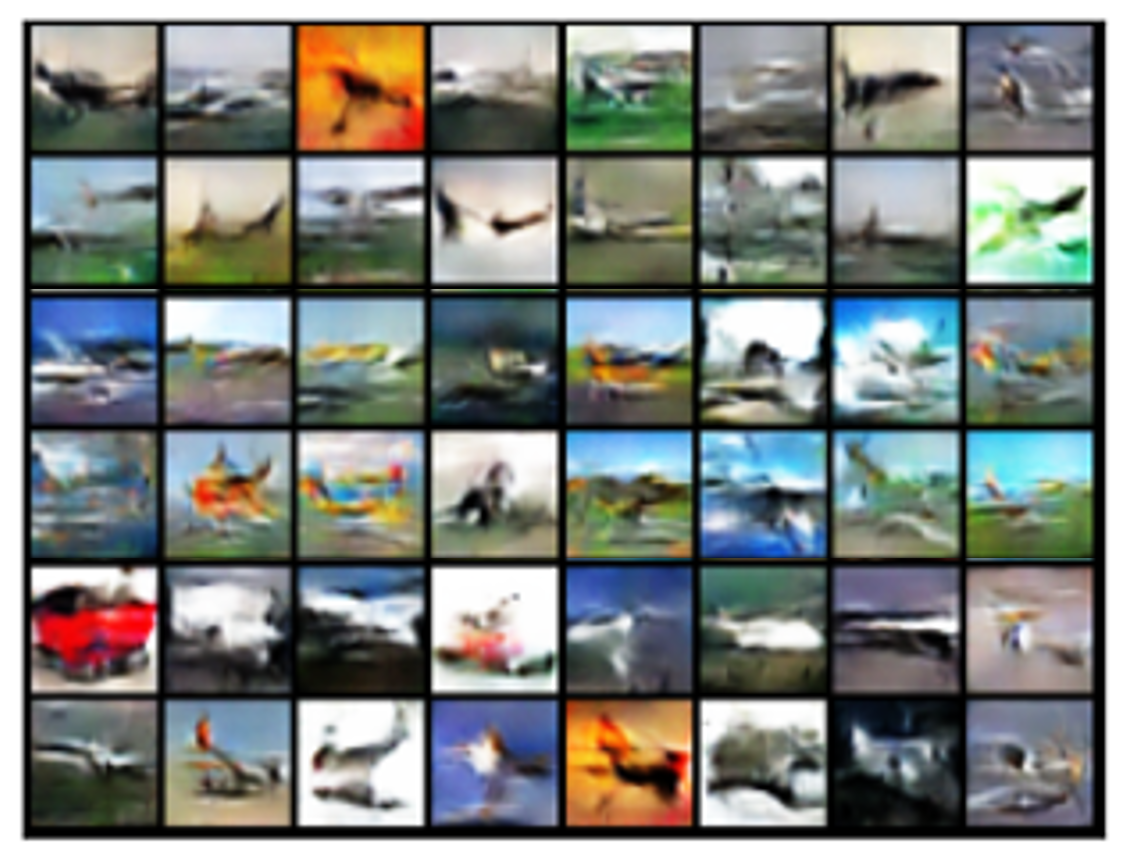
\includegraphics[width=0.41\textwidth]{\toplevelprefix/chapters/chapter5/figs/memory_before_review_clip.png}
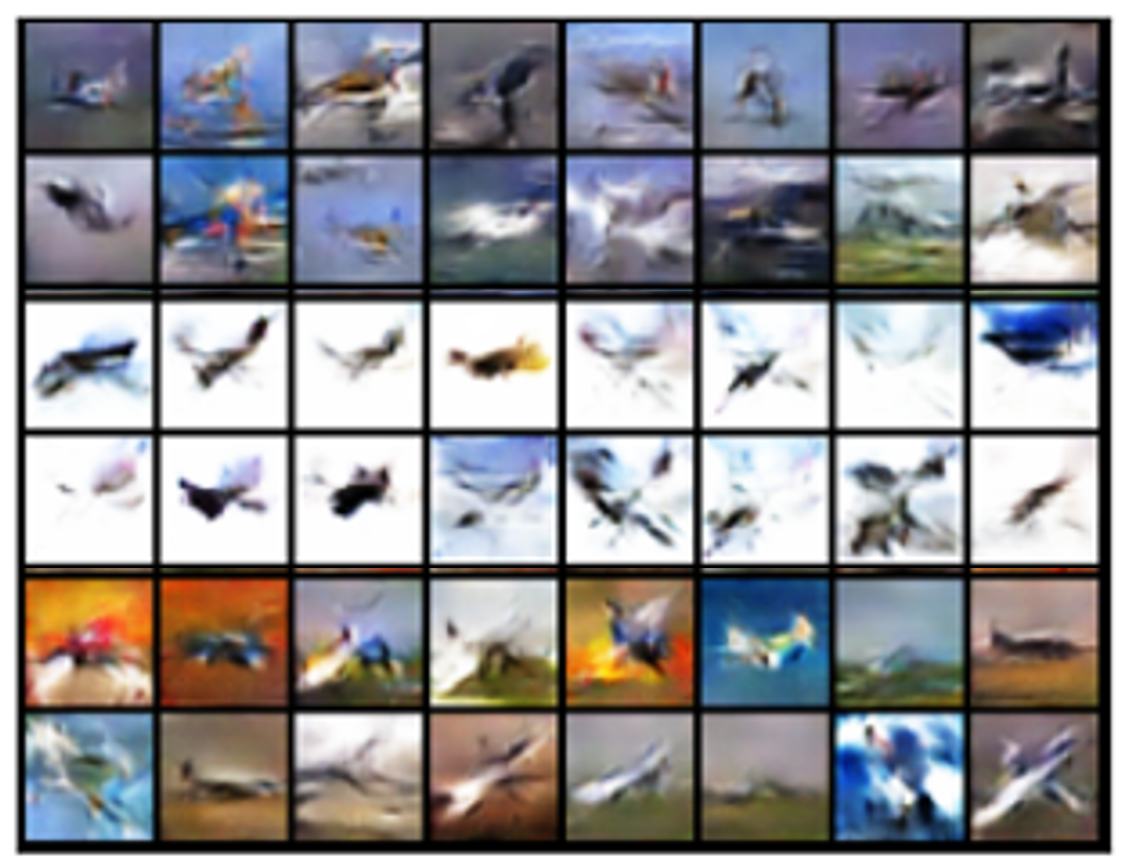
\includegraphics[width=0.4\textwidth]{\toplevelprefix/chapters/chapter5/figs/memory_after_review_clip.png}
 \caption{\small Visualization of replayed images $\hat{\x}_{old}$ of class 1-`airplane' in CIFAR-10, before (left) and after (right) one reviewing cycle.} 
\label{fig:memory_review}
\end{figure}


\subsection{Sample-wise Continuous Unsupervised Learning}
\label{sec:sample-wise-incremental}
%This subsection shows that the closed-loop architecture is applicable to \href{https://arxiv.org/abs/2210.16782}{sample-wise continuous learning}, probably even with white-box backbone networks.

As we know, the closed-loop CTRL formulation can already learn a decent autoencoding, even without class information, with the  CTRL-Binary program:
\begin{align}
      \max_\theta \min_\eta \quad \Delta R(\Z, \hat{\Z}) 
 \label{eqn:CTRL-Binary}
\end{align}
However, note that \eqref{eqn:CTRL-Binary} is practically limited because it only aligns the dataset $\X$ and the regenerated $\hat \X$ at the distribution level. 
There is no guarantee that for each sample $\x$ would be close to the decoded $\hat \x = g(f(\x))$. 

\paragraph{Sample-wise constraints for unsupervised transcription.} 
\label{sec:constraints}
To improve discriminative and generative properties of representations learned in the unsupervised setting, we propose two additional mechanisms for the above CTRL-Binary maximin game \eqref{eqn:CTRL-Binary}.  For simplicity and uniformity, here these will be formulated as equality constraints over rate reduction measures, but in practice they can be enforced softly during optimization.

\paragraph{Sample-wise self-consistency via closed-loop transcription.} 
First, to address the issue that CTRL-Binary does not learn a sample-wise consistent autoencoding, we need to promote $\hat \x$ to be close to $\x$ for each sample. In the CTRL framework, this can be achieved by enforcing their corresponding features $\z=f(\x)$ and $\hat \z = f(\hat \x)$ to be close. 
To promote sample-wise self-consistency, where $\hat{\x} = g(f(\x))$ is close to $\x$ , we want the distance between $\z$ and $\hat{\z}$ to be zero or small, for all $N$ samples.
This distance can be measured by the rate reduction:
\begin{align}
\sum_{i\in N} \Delta R(\z^i,\hat{\z}^i) = 0.
\label{eqn:sample-self-consistency}\vspace{-2mm}
\end{align}
Note that this again avoids measuring differences in the image space.

\paragraph{Self-supervision via compressing augmented samples.} 
Since we do not know any class label information between samples in the unsupervised settings, the best we can do is to view every sample and its augmentations (say via translation, rotation,  occlusion etc) as one ``class'' --- a basic idea behind almost all self-supervised learning methods. In the rate reduction framework, it is natural to compress the features of each sample and its augmentations. In this work, we adopt the standard transformations in SimCLR \cite{chen2020simple} and denote such a transformation as $\tau$. We denote each augmented sample $\x_a = \tau(\x)$, and its corresponding feature as $\z_a = f(\x_a, \theta) $. For discriminative purposes, we hope the classifier is {\em invariant} to such transformations. Hence it is natural to enforce that the features $\z_a$ of all augmentations are the same as that $\z$ of the original sample $\x$. This is equivalent to requiring the distance between $\z$  and  $\z_a$, measured in terms of rate reduction again, to be zero (or small) for all $N$ samples: 
\begin{align}
\sum_{i\in N} \Delta R(\z^i,\z_{a}^i) = 0.
\label{eqn:sample-compression}\vspace{-3mm}
\end{align}


\paragraph{Unsupervised representation learning via closed-loop transcription.} 
So far, we know the CTRL-Binary objective $\Delta R(\Z, \hat{\Z})$ in \eqref{eqn:CTRL-Binary} helps align the distributions while sample-wise self-consistency \eqref{eqn:sample-self-consistency} and sample-wise augmentation \eqref{eqn:sample-compression} help align and compress features associated with each sample. Besides consistency, we also want learned representations are maximally discriminative for different samples (here viewed as different ``classes''). Notice that the rate distortion term $R(\Z)$ measures the coding rate (hence volume) of all features. %It has been observed in \cite{li2022neural} that by maximizing this term, learned features expand and hence become more discriminative. 

\paragraph{Unsupervised CTRL.} Putting these elements together, we propose to learn a representation via the following constrained maximin program, which we refer to as {\em unsupervised CTRL} (u-CTRL):
\begin{align}
      \max_\theta \min_\eta  \quad & R(\Z) + \Delta R(\Z, \hat{\Z}) \label{eqn:constrained_maxmin}\\
 \mbox{subject to} \quad & \sum_{i\in N} \Delta R(\z^i, \hat{\z}^i) = 0, \;\; \mbox{and} \;\; \sum_{i\in N} \Delta R(\z^i, \z_{a}^i) = 0. \nonumber
\end{align}
Figure \ref{fig:framework-uCTRL} illustrate the overall architecture of the closed-loop system associated with this program.
\begin{figure}[t]
\centering
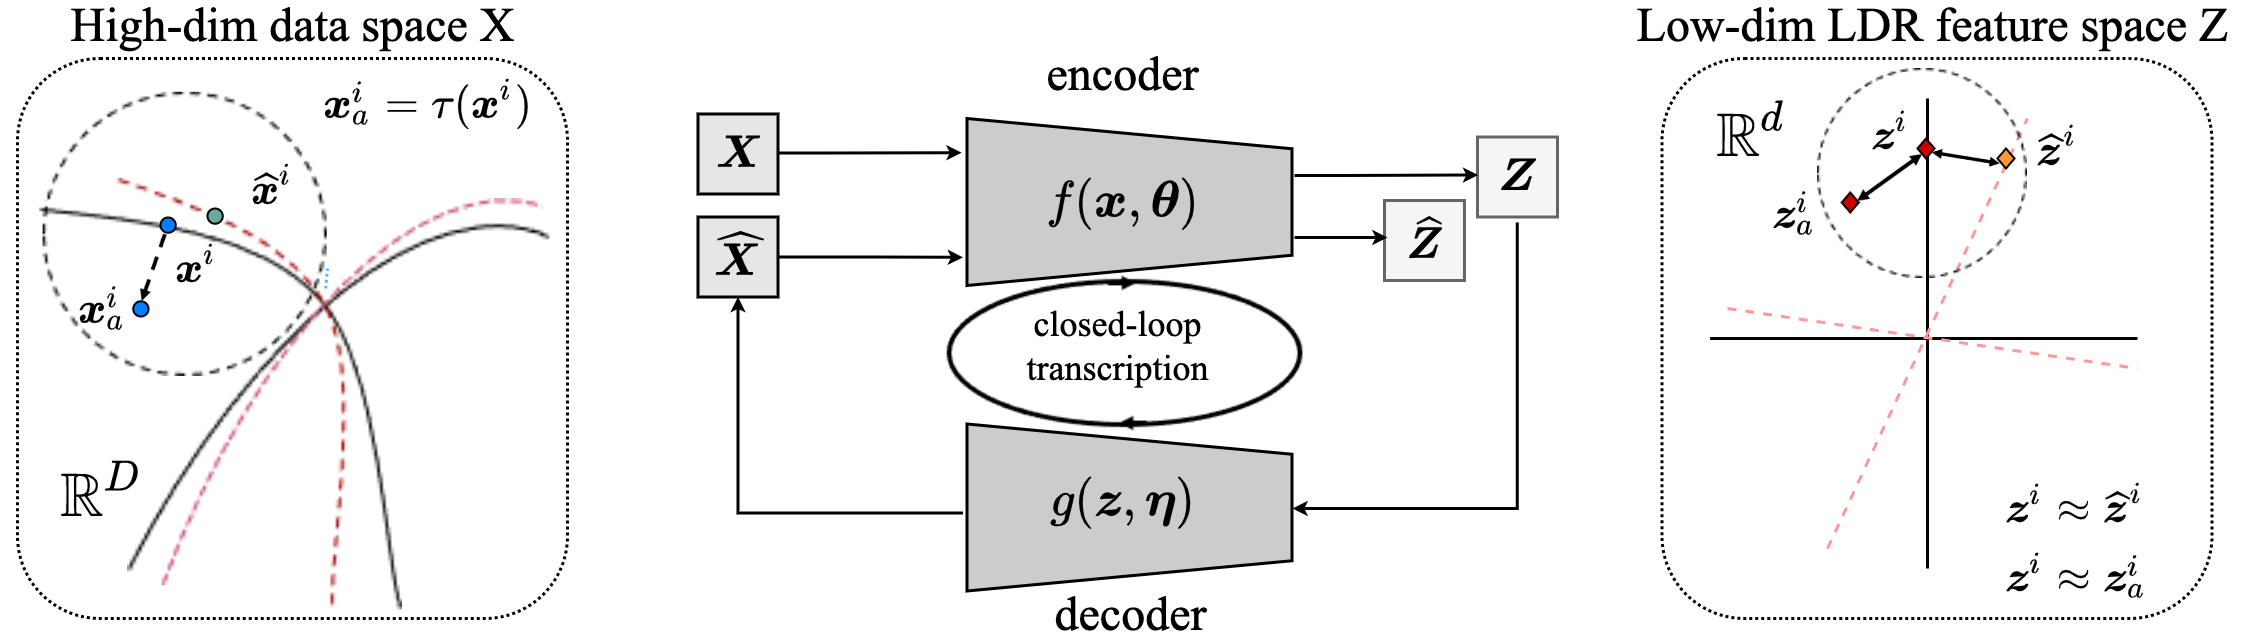
\includegraphics[width=0.98\textwidth]{\toplevelprefix/chapters/chapter5/figs/uCTRLv3.png}
\caption{\textbf{Overall framework} of closed-loop transcription for unsupervised learning. Two additional constraints are imposed on the Binary-CTRL method: 1) self-consistency for sample-wise features $\z^i$ and $\hat{\z}^i$, say $\z^i \approx \hat{\z}^i$; and 2) invariance/similarity among features of augmented samples $\z^i$ and $\z_{a}^i$, say $\z^i \approx \z_{a}^i=f(\tau(\x^i), \theta)$, where $\x^i_a=\tau(\x^i)$ is an augmentation of sample $\x^i$ via some transformation $\tau(\cdot)$.}
\label{fig:framework-uCTRL}
\end{figure}

In practice, the above program can be optimized by alternating maximization and minimization between the encoder $f(\cdot,\theta)$ and the decoder $g(\cdot,\eta)$. We adopt the following optimization strategy that works well in practice, which is used for all subsequent experiments on real image datasets:
\vspace{-1mm}
\begin{align}
  &  \max_{\theta}\; R(\Z) + \Delta{R(\Z, \hat{\Z})-\lambda_{1}\sum_{i\in N} \Delta R(\z^i, \z_{a}^i)} -\lambda_{2}\sum_{i\in N} \Delta R(\z^i, \hat{\z}^i) \label{eqn:constrained_max}; \\
% \end{align}
% \begin{align}
   & \min_{\eta}\; R(\Z) + \Delta{R(\Z, \hat{\Z})+\lambda_{1}\sum_{i\in N} \Delta R(\z^i, \z_{a}^i)+ \lambda_{2}\sum_{i\in N} \Delta R(\z^i, \hat{\z}^i)} \label{eqn:constrained_min}, 
\end{align}
where the constraints $\sum_{i\in N} \Delta R(\z^i, \hat{\z}^i) = 0$ and $\sum_{i\in N} \Delta R(\z^i, \z_{a}^i) = 0$ in \eqref{eqn:constrained_maxmin} have been converted (and relaxed) to Lagrangian terms with corresponding coefficients $\lambda_{1}$ and  $\lambda_{2}$.\footnote{Notice that computing the rate reduction terms $\Delta R$ for all samples or a batch of samples requires computing the expensive $\log\det$ of large matrices. In practice, from the geometric meaning of $\Delta R$ for two vectors, $\Delta R$ can be approximated with an $\ell^2$ norm or the cosine distance between two vectors.}

The above representation is learned without class information. In order to facilitate discriminative or generative tasks, it must be highly structured. It has been verified experimentally that this is indeed the case and u-CTRL demonstrates significant advantages over other incremental or unsupervised learning methods \cite{pmlr-v234-tong24a}. We here only illustrate some qualitative results with the experiment on the CIFAR-10 dataset \cite{krizhevsky2014cifar}, with standard augmentations for self-supervised learning \cite{chen2020simple}. One may refer to \cite{pmlr-v234-tong24a} for experiments on more and larger datasets and their quantitative evaluations. 

As one can see from the experiments, specific and unique structure indeed emerges naturally in the representations learned using u-CTRL: globally, features of images in the same class tend to be clustered well together and separated from other classes, as shown in Figure \ref{fig:heatmap_z}; locally, features around individual samples exhibit approximately piecewise linear low-dimensional structures, as shown in Figure \ref{fig:tsne}. 

\begin{figure}[t]
     \footnotesize
     \centering
    % \subfigure[CIFAR-10]{
    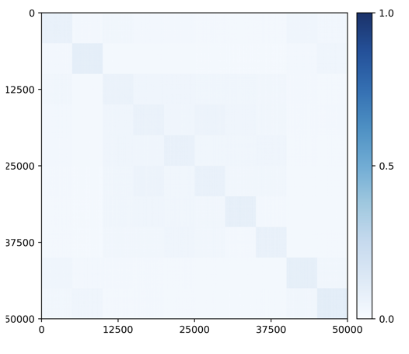
\includegraphics[width=0.5\textwidth]{\toplevelprefix/chapters/chapter5/figs/CIFAR10_cifar10_heatmap_zz.png}
    % }
    %  \subfigure[CIFAR-100]{
    %      \includegraphics[width=0.305\textwidth]{CIFAR100_cifar100_heatmap.png}
    %  }
    %  \subfigure[Tiny ImageNet]{
    %      \includegraphics[width=0.305\textwidth]{tinyimagenet_heatmap.png}
    %  }
    % \vspace{-0.15in}
    \caption{\small Emergence of block-diagonal structures of $|\Z^\top \Z|$ in the feature space for CIFAR-10.}
    \label{fig:heatmap_z}
\end{figure}

\begin{figure}[ht!]
    \begin{subfigure}[t]{0.46\textwidth}
        \centering
        \includegraphics[width=\textwidth]{\toplevelprefix/chapters/chapter5/figs/uCTRL-tsne2.png}
        \caption{u-CTRL}
    \end{subfigure}
    \hfill
    \begin{subfigure}[t]{0.46\textwidth}
        \centering
        \includegraphics[width=\textwidth]{\toplevelprefix/chapters/chapter5/figs/MoCoV2-tsne3.png}
        \caption{MoCoV2}
    \end{subfigure}
    %  \footnotesize
    %  \centering
    %  \subfigure[u-CTRL]{
    %      \includegraphics[width=0.46\textwidth]{chapters/chapter5/figs/uCTRL-tsne2.png}
    %  }
    %  \subfigure[MoCoV2]{
    %      \includegraphics[width=0.46\textwidth]{chapters/chapter5/figs/MoCoV2-tsne3.png}
    %  }
    \caption{\small t-SNE visualizations of learned features of CIFAR-10 with different models.} 
    \label{fig:tsne}
\end{figure}

\paragraph{Unsupervised conditional image generation via rate reduction.}
The highly-structured feature distribution also suggests that the learned representation can be very useful for generative purposes. For example, we can organize the sample features into meaningful clusters, and model them with low-dimensional (Gaussian) distributions or subspaces. By sampling from these compact models, we can conditionally regenerate meaningful samples from computed clusters. This is known as {\em unsupervised conditional image generation} \cite{hwang2021stein}. 

To cluster features, we exploit the fact that the rate reduction framework \eqref{eqn:maximal-rate-reduction} is inspired by unsupervised clustering via compression \cite{ma2007segmentation}, which provides a principled way to find the membership $\bm \Pi$.
Concretely, we maximize the same rate reduction objective \eqref{eqn:maximal-rate-reduction} over $\bm \Pi$, but fix the learned representation $\Z$ instead. We simply view the membership $\bm \Pi$ as a nonlinear function of the features $\Z$, say $h_{\bm \pi}(\cdot,\xi):\Z \mapsto \bm \Pi$ with parameters $\xi$. In practice, we model this function with a simple neural network, such as an MLP head right after the output feature $\z$. 
To estimate a ``pseudo'' membership $\hat{\bm \Pi}$ of the samples, we solve the following optimization problem over $\bm \Pi$:
\begin{align}
    \hat{\bm \Pi} = \arg\max_{\xi} \Delta R(\Z| \bm \Pi(\xi)).
\label{eqn:cluster_mcr}
\end{align}
In Figure \ref{fig:vis_clustering}, we  visualize images generated from the ten unsupervised clusters from \eqref{eqn:cluster_mcr}. Each block represents one cluster and each row represents one principal component for each cluster. Despite learning and training without labels, the model not only organizes samples into correct clusters, but is also able to preserve statistical diversities within each cluster/class. We can easily recover the diversity within each cluster by computing different principal components and then sample and generate accordingly. While the experiments presented here are somewhat limited in scale, we will explore more direct and powerful methods that utilize the learned data distributions and representations for conditional generation and estimation in the next chapter.
\begin{figure}[t]
    \footnotesize
    \centering
    \includegraphics[width=0.95\textwidth]{\toplevelprefix/chapters/chapter5/figs/CIFAR10_generatedfromcluster.png}
    \caption{\small Unsupervised conditional image generation from each cluster of CIFAR-10, using u-CTRL. Images from different rows mean generation from different principal components of each cluster.}
    \label{fig:vis_clustering}
\end{figure}




% \section{Other Variations} 
% to be determined...

\section{Summary and Notes}
Materials presented in this chapter are based on a series of recent work on this topic: \cite{Dai-entropy-2022}, 
\cite{pai2022pursuit}, \cite{tong2023incremental}, and \cite{pmlr-v234-tong24a}. In particular, Section \ref{sec:closed-loop-transcription} is based on the pioneering work of \cite{Dai-entropy-2022}. After that, the work of \cite{pai2022pursuit} has provided strong theoretical justifications for the closed-loop framework, at least for an ideal case. Section \ref{sec:class-wise-incremental} and Section \ref{sec:sample-wise-incremental} are based on the works of \cite{tong2023incremental} and \cite{pmlr-v234-tong24a}, respectively. They demonstrate that the closed-loop framework naturally supports incremental and continuous learning, either in a class-wise or sample-wise setting. The reader may refer to these papers for more technical and experimental details.


\paragraph{Shallow vs.\ deep neural networks, for autoencoding and more.}
In \Cref{sub:nonlinear-pca}, we discussed Cybenko's universal approximation
theorem and how it states that in principle, a neural network with a single
hidden layer (and suitable elementwise nonlinearities) is sufficient to
approximate any suitably regular target function. Of course, in practice, the
major architectural reason for the dominance of neural networks in practice has
been the refinement of techniques for training \textit{deeper} neural networks.
Why is depth necessary?
From a fundamental point of view, the issue of depth separations, which
construct settings where a deeper neural network can approximate a given class
of target functions with exponentially-superior efficiency relative to a shallow
network,
has been studied at great length in the theoretical literature:
examples include \cite{Telgarsky2016-sn,Bresler2020-xy,Venturi2021-qc}. 
The ease of training deeper
networks in practice has not received as satisfying of an answer from the
perspective of theory. 
ResNets \cite{he2016deep} represent the pioneering empirical work of
making deeper networks more easily trainable, used in nearly all modern
architectures in some form. Theoretical studies have focused heavily on
trainability of very deep networks, quantified via the initial neural tangent
kernel \cite{Buchanan2021-sj,Martens2021-cx}, but these studies have not given
significant insight into the trainability benefits of deeper networks in middle
and late stages of training (but see \cite{Yang2021-gw} for the root of a line
of research attempting to address this).

\section{Exercises and Extensions}

\end{document}
